\chapter{Brotas: fronteira do urbano em Salvador}\label{cap:2}

Uma das epígrafes desta dissertação o indica com certo espanto: Brotas antes da Primeira República era uma freguesia -- assim se chamavam os \textit{distritos} antes da separação entre igreja e Estado -- eminentemente rural. Em 1930, entretanto, encontramos Brotas como um distrito razoavelmente urbanizado, com novos núcleos populacionais estabelecidos e usos do solo muito diversificados, indo da residência proletária ao veraneio burguês; das roças às fábricas; das casas de taipa, telheiros e barracões aos palacetes e chalés ecléticos. Estaria nos conflitos sociais a chave para a compreensão desta mudança de perfil, como tenho afirmado até o momento?

O capítulo anterior foi totalmente dedicado à compreensão do contexto socioeconômico global, nacional, estadual e municipal do período analisado, num momento \textit{sincrônico} da exposição da presente pesquisa. Foi possível esboçar, desta forma, um quadro explicativo dos conflitos sociais constituintes do território soteropolitano durante a Primeira República (1889-1930), com algumas de suas muitas determinantes. A passagem deste ponto para a análise dos conflitos sociais responsáveis pela produção, apropriação e uso do espaço urbano de Brotas pede, entretanto, uma mediação, pois os conflitos sociais, do modo como são aqui compreendidos, são \textit{dinâmicos}, só se deixam perceber em análise \textit{diacrônica}, e a passagem do tempo pressupõe obviamente um ``antes'' e um ``depois''. É hora, portanto, de entender o ``antes'' territorial de Brotas, preparando, com esta análise das conjunturas espaciais pretéritas do distrito, o terreno para a análise dos processos de produção, apropriação e uso do território do distrito no período estudado. 

Eis aqui, portanto, um \textit{segundo vetor} de compreensão dos conflitos sociais e de sua influência sobre a produção, apropriação e uso do território do distrito; se o primeiro foi o \textit{enquadramento sincrônico} num contexto, para percebermos as influências contemporâneas externas ao território, trata-se agora de perceber as \textit{contradições internas em processo}, para que o território e sua produção, apropriação e uso resultem da confluência entre as influências externas e as contradições internas. Para caracterizar este segundo vetor será preciso fazer, em primeiro lugar, um breve histórico da formação e delimitação territorial da freguesia de Brotas; em seguida, as características socioeconômicas desta freguesia serão descritas em traços largos; outros usos porventura não explicitados do seu espaço serão delimitados e caracterizados; por último, se tentará capturar o retrato que os soteropolitanos de outros distritos faziam de Brotas. 

Antes de prosseguir, duas digressões derivadas de uma observação. A escassez de fontes não é problema da História, mas do historiador e de suas próprias limitações. A ele cabe resolver criativamente a questão, seja empregando a documentaçao disponivel para estabelecer cenários factíveis, a partir dos quais extrair esboços descritivos, pendentes de maiores estudos, seja inventando novos meios de torcionar as fontes até que confessem o que deseja.

Esta questão aplica-se perfeitamente à reconstrução da história fundiária e dos conflitos sociais ocorridos em Brotas. Embora simples de descrever em traços largos -- e.g., ``Brotas é um distrito eminentemente rural, onde herdades e fazendolas eram os limites extremos das formas de ocupação territorial encontradas'', ou qualquer outra generalização apressada do tipo --, a tarefa torna-se verdadeiro desafio se levada aos menores detalhes, pois o Arquivo Público do Estado da Bahia custodia entre seus documentos apenas um livro de registro de terras desta freguesia\footnote{BR BAAPB, fundo Colonial, série Registros de Terra, livro 4675.}, que tanto pode ser o remanescente de uma série, a julgar pelo que se pode encontrar relativamente a outras freguesias e paróquias no mesmo Arquivo, quanto pode ser o resultado de enorme desleixo dos párocos; a primeira hipótese parece ser a mais plausível. Este livro de terras -- ao que tudo indica único já primeira metade dos anos 1980, quando uma das mais conhecidas diretoras do Arquivo Público da Bahia escreveu seu livro sobre as freguesias urbanas de Salvador \cite{NASCIMENTO2007} --, é a peça central em torno da qual se tentará esboçar daqui em diante, com apoio de outras fontes, uma caracterização fundiária da freguesia de Brotas no século XIX. 

O método mais adequado para burilar e esmerilar este esboço, fazendo dele obra acabada, é simples, mas trabalhoso. Primeiro, listar os nomes de proprietários, posseiros, arrendatários e quantos mais houver no livro de registro de terras remanescente e, em seguida, vasculhar seus inventários, estabelecendo assim árvores genealógicas; paralelamente, usar os nomes constantes nestas listas e nas cadeias sucessórias que se forem formando para escarafunchar tanto os inventários quanto notas de tabeliães e outros livros de escrituras mais recentes em busca dos bens destas pessoas. Ocorre que, embora seja possível reconstruir a história fundiária da freguesia de Brotas (ou qualquer outra) usando este método, há dois impedimentos à sua adoção na presente pesquisa: nem há tempo disponível para a empreitada nos prazos de uma pesquisa de mestrado, nem o recorte temporal escolhido autoriza fazer pesquisa minuciosa em período anterior ao 15 de novembro de 1889. Será suficiente, para esta etapa da pesquisa, investigar \textit{alguns} dos proprietários de terras, não todos\footnote{A lista com todos os nomes constantes no \textbf{Livro Eclesial de Registro de Terras da Freguesia de Brotas} encontra-se no}; se a análise densa da composição fundiária do território não é possível nem recomendada neste momento, é possível, entretanto, estabelecer padrões e tendências, e assim preparar o terreno para a análise que se fará no capítulo seguinte, baseada esta em livros de registro das décimas urbanas selecionados e na análise da totalidade dos pedidos de licença de obras para este distrito.

Situação ainda mais difícil é a da análise dos conflitos sociais no distrito ao longo de três séculos de história (1549-1889), agravada pelo fato de Brotas ser uma vasta freguesia semi-rural, quase inexplorada historiograficamente; \textit{hic sunt dracones}, é o que certamente escreveriam cartógrafos da era dos descobrimentos sobre os mapas de Brotas se deste distrito tivessem se ocupado. Alarga-se, aqui, um debate travado por um historiador italiano, que ridicularizou a ``artificiosa concentração da historicidade intrínseca da cidade no núcleo antigo'' \cite[p.~74]{argan_histcid_1992}; sua polêmica, entretanto, foi contra a oposição ``absurda'' entre uma ``cidade antiga'' e uma ``cidade moderna'' conceitualmente apartadas, pois 

\begin{citacao}
\dots se se quer conservar a cidade como instituição, não se pode admitir que ela conste de uma parte histórica com um valor qualitativo e de uma parte não-histórica, com caráter puramente quantitativo. Fique bem claro que o que tem e deve ter não apenas organização, mas substância histórica é a cidade em seu conjunto, antiga e moderna. Pôr em discussão sua historicidade global equivale a pôr em discussão o valor ou a legitimidade histórica da sociedade contemporânea, o que talvez alguns queiram, mas que o historiador não pode aceitar \cite[p.~79]{argan_histcid_1992}.
\end{citacao}

O desenvolvimento da pesquisa exposta nesta dissertação evidenciou outro lado da questão. Embora os efeitos desta distinção ``absurda'' aparentemente se produzam no presente e a ele se circunscrevam, eles reverberam sobre o passado pela influência exercida sobre as agendas de pesquisa historiográfica, resultando, no caso que nos interessa mais de perto, em inflação de produtos acadêmicos acerca do \textit{centro histórico} de Salvador e num silêncio ensurdecedor quanto às zonas \textit{suburbana} e \textit{rural} da cidade. 

Como as ondas a irradiar de uma pedra atirada à água, os reflexos deste erro se multiplicam: se a produção historiográfica sobre o território soteropolitano se concentra no estudo da área mais densamente povoada, em especial nas freguesias propriamente urbanas e nas semi-rurais que as rodeavam (Santo Antônio, Vitória, Brotas), resulta disso que a historiografia dos bairros populares de Salvador surgidos da década de 1940 em diante no território destes distritos suburbanos e rurais toma como marco zero a primeira grande ``invasão'' coletiva de terras, que se disputa ter sido a da Vila Ruy Barbosa, a de Gingibirra ou a do Corta-Braço; toda a produção, apropriação e uso anterior destes territórios, inclusive por sujeitos históricos muito semelhantes aos ``invasores'' em seu respectivo contexto, resta condenada ao oblívio. É como se, negados os seus direitos mais básicos por décadas, os sujeitos históricos construtores destes territórios populares -- sejam os do século XX, sejam seus antepassados --  tivessem negado também o seu direito à representação histórica, ao status de agentes construtores da História tão legítimos quanto qualquer outro.

Foi com certo esforço que encontrei referências à freguesia de Brotas nas mais renomadas obras de conjunto sobre a Bahia dezenovista \cite{MATTOSO1978, MATTOSO1992, NASCIMENTO2007}, e numa delas, embora dedicada à análise pormenorizada das freguesias urbanas da cidade, nem sempre foi possível contar com a documentação necessária para se chegar aos melhores resultados \cite{NASCIMENTO2007}. Um historiador da \textit{longue durée} menciona timidamente o distrito nalgumas páginas de sua obra maior \cite{tavares_historia_2008}, e embora um geógrafo tenha se ocupado pontuadamente da evolução territorial do distrito numa de suas duas obras maiores \cite{VASCONCELOS2002}. 

Para superar de forma rápida a lacuna, fez-se necessário o recurso a instrumentos digitais de pesquisa como a \textbf{Hemeroteca Digital Brasileira}, a \textbf{Biblioteca Brasiliana Guita e José Mindlin}, o \textbf{Internet Archive} e os \textbf{Anais da Biblioteca Nacional}. Mesmo sabedor das limitações de tais fontes arquivísticas digitais, pois trata-se de coleções de impressos (jornais, revistas, livros, panfletos etc.) que não pretendem nem podem suprir arquivos físicos custodiadores de documentação de outra natureza (processos judiciais, registros de terras, correspondências etc.), os resultados foram impressionantes. Foi possível, em alguns casos, chegar a conclusões bastante seguras acerca de alguns fatos, e noutros foi possível estabelecer com maior precisão datas e circunstâncias de fatos que de outra maneira ficariam abertos à especulação; mesmo nos casos em que as fontes consultadas não permitiram chegar a qualquer conclusão definitiva, foi possível construir hipóteses plausíveis, ou mesmo delimitar o campo de possibilidades a um leque mais restrito.

Que os resultados, portanto, falem por si. Eis, então, uma história de como se formou o distrito de Brotas antes da Primeira República.

\section{Fundação e delimitação territorial da freguesia}\label{sec:2.1}

\subsection{Dos tempos pré-cabralinos à fundação da freguesia}\label{subsec:precabral}

A primeira notícia que se tem de qualquer forma de povoação do território que viria a compor a freguesia de Brotas remete à existência, muito provavelmente pré-cabralina, das aldeias tupinambás que viriam a ser conhecidas como \index{Mariquita!Mairiquiig (aldeia)}\textit{Mairaqui}, ou \textit{Mairiquiig}, de onde deriva o nome do atual \index{Mariquita!largo da}\textit{largo da Mariquita}, e que significa, em tupi, ``naufrágio dos franceses''; \index{Ubarana!aldeia da}\textit{Ubarana}, muito provavelmente no lugar onde se situou a fazenda cujos limites serão descritos adiante; e \index{Pituba!aldeia da}\textit{Pituba}, no bairro que hoje leva o mesmo nome \cite{azevedo_povoamento_1969,dorea_ruas_1999,sampaio_salvador_2016,VASCONCELOS2002}...\footnote{Tomar a cesura cabralina e a invasão colonial portuguesa como ponto de partida soará, como no caso das estatísticas populacionais urbanas globais da \autoref{tab:pop100mundo}, \textit{colonialista}. Serve aqui a mesma advertência anterior, acrescida do fato de que, com o extermínio ou sujeição das aldeias circunvizinhas a Salvador durante o governo-geral de Mem de Sá, qualquer registro ou memória mais aprofundado ou detalhado sobre a dinâmica populacional destes assentamentos humanos tupis foi destruída, restando deles, infelizmente, apenas menções pontuais na obra de cronistas.}. Da parte dos colonizadores portugueses, a primeira notícia que se tem é a de um engenho, existente na localidade hoje conhecida como Engenho Velho, segundo algumas fontes, já no período anterior à chegada de Tomé de Souza em 1549 \cite[p.~235]{sampaio_salvador_2016}.

Após o estabelecimento da cabeça-de-ponte portuguesa na Conceição da Praia e a construção, entre 1549 e 1551, das primeiras edificações e muros no cume da falha geológica soteropolitana, onde hoje se localiza a Praça Municipal, ainda se fazia necessário para estes primeiros portugueses, por questão de sobrevivência mesmo, submeter o ``gentio'' a seu domínio\footnote{Não se pode interpretar de outro modo instruções constantes no Regimento de Tomé de Souza como a de tomar posse da antiga Vila do Pereira, à força se necessário (item 3 do Regimento); localizar os tupinambás, distinguir entre eles os dispostos à paz para alianças e os dispostos à guerra para os castigar, ``destruindo-lhes suas aldeias e povoações, matando e cativando aquela parte deles que vos parecer que basta para seu castigo e exemplo de todos'' e mandando enforcar os chefes nas suas respectivas aldeias (item 6 do Regimento); em tomada a Vila do Pereira, construir imediatamente uma fortaleza e povoação em lugar mais para dentro da Baía de Todos os Santos, em ``sítio sadio e de bons ares'' com ``abastança de águas e porto'', apta a prover as outras capitanias (item 8 do Regimento), com seis léguas de termo para cada lado (item 9 do Regimento). Além da sujeição pela força, a ordem dada a Tomé de Souza quanto às relações com os tupinambás era de conceder a paz aos assim submissos, desde que eles ``reconheçam sujeição e vassalagem, com encargo de darem em cada ano alguns mantimentos para a gente da povoação'' \cite[pp.~81-101]{ruy_politica_1949}.}.

Secular tradição política europeia recomendava a soberanos, senhores e magnates, ao menos desde a Idade Média e nos territórios onde vigeu plenamente o regime senhorial, estabelecer igrejas paroquiais como instrumento para aglutinação populacional e exercício de soberania \cite[pp.~193-205]{BERNARDO1997}. O rei português João III, sabedor e praticante desta tradição, ordenou no seu Regimento a Tomé de Souza replicá-la por estas bandas, adaptando-a às novas circunstâncias: neste documento, levou em conta o ``grande inconveniente'' de se fazer os índios convertidos morar na terra de outros índios não-cristãos e de permitir qualquer contato entre uns e outros. Por isto, recomendou expressamente trazer os índios cristianizados para perto das povoações portuguesas (item 45 do Regimento). A forma encontrada para isolar os recém-convertidos e submetê-los à soberania portuguesa, quebrando seus padrões culturais ao tempo em que se lhes impunham os hábitos e costumes reinóis, foi a criação dos \textit{aldeamentos}, comunidades indígenas tuteladas por colonos ou padres \cite[pp.~72-76]{santos_salvador_2004}.

Justo a primeira experiência de aldeamento conduzida pelos portugueses foi a povoação de \textit{São Paulo}. Em carta datada de 5 de julho de 1559, Manuel da Nóbrega, que dá a esta comunidade religiosa primazia entre outras três criadas depois da chegada do governador-geral Mem de Sá em 1557\footnote{As outras são as de \textit{São João}, ``a três léguas da cidade'', e a de \textit{Sancti Spiritus} (ou \textit{Espírito Santo}, a ``sete léguas''. A primeira localizava-se próximo ao atual bairro soteropolitano de Plataforma, e a última deu início à povoação de Abrantes, em Camaçari.}, descreve em breves linhas sua rotina, mas não sua forma: diz que ali já estava instalada uma escola de meninos, com algo entre oitenta e cento e vinte alunos que estudavam à tarde, ``porque tem o mar longe e vão pelas manhãs pescar para si e para seus pares que não se mantêm d'outra coisa''; estes jovens eram encarregados pelos jesuítas de catequizar seus pais e os mais velhos à noite, depois dos estudos \cite[p.~179]{nobrega_cartas_1931}. Afirma-se que este aldeamento localizava-se, tomando como base marcos atuais, ou no Alto do Cruzeiro (no atual bairro de Cosme de Farias), ou no Largo da Cruz da Redenção \cite[p.~87]{campos_brotas_1942}.

Este aldeamento se constituiu à base de índios trazidos das aldeias do Rio Vermelho e arredores --- e o Rio Vermelho foi outro núcleo populacional importante da freguesia, existente mesmo antes de sua constituição\footnote{Como se verá adiante, trata-se do trecho do Rio Vermelho que, usando marcos atuais, está compreendido entre a foz do rio Lucaia e a praça dos Jangadeiros, em frente ao Quartel de Amaralina. O trecho do bairro do Rio Vermelho situado entre a praia da Paciência e a foz do rio Lucaia pertenceu, desde sempre, à freguesia da Vitória.}. Esta localidade tem registros históricos que remontam ao século XVI, e apontam para povoação ainda mais recuada no tempo: cabe registrar a existência de aldeias e aldeamentos no Morro do Conselho (aldeamento de Nossa Senhora do Rio Vermelho) e proximidades (aldeamento de São Lourenço, ou Tamandaré) \cite[p.~75]{santos_salvador_2004}.

Ao contrário do que afirma a historiografia clássica sobre a invasão holandesa a Salvador (1624-1625), nem o Morro do Conselho, nem a localidade onde se situa o atual bairro do Rio Vermelho foram usados como refúgio pelos portugueses durante a invasão holandesa de 1624-1625. O rio Camarajipe, um dos principais a cortar o território soteropolitano, teve seu nome vertido para o português como ``rio vermelho'' em função da abundância em suas margens do \textit{camará vermelho}, ou \textit{lantana}, planta de flor vermelha. O Camarajipe, antes de lhe imporem mudanças ao leito, nascia próximo da enseada do Lobato, na Boa Vista, e confluía com o Lucaia para desembocar num estuário comum, onde hoje é o largo da Mariquita; desde 1866 o Camarajipe passou a correr por baixo da Estrada do Retiro, atual Avenida San Martin, e assim perdeu-se, com o tempo, a noção de que o ``rio vermelho'' atravessa o território soteropolitano em sentido latitudinal desde o mar interno da Baía de Todos os Santos até as praias atlânticas. Quanto ao  ``arraial do Rio Vermelho'', reduto dos portugueses na luta contra os holandeses, há vários indícios históricos de que foi na verdade construído onde hoje fica o \textit{largo do Tanque}, na altura do que deveria ser, à época, o tanque do engenho Conceição\footnote{\citeonline{edelweiss_camarajipe_1969}, que aponta a tradução do tupi para o português, credita tudo isto a uma confusão linguística. Sobre a construção do ``arraial do Rio Vermelho'' no atual Largo do Tanque, cujo nome teria induzido a historiografia a erro quanto à sua real localização, cf. \citeonline[p.~54-62]{magalhaes_equus_2010}, que usa conhecimento apurado do sistema de medidas de época e indícios documentais para situar o arraial. Para visualizar o leito do Camarajipe antes do tamponamento, assim como a proximidade entre uma das nascentes do Camarajipe e o tanque do Engenho Conceição, cf. o mapa de \citeonline{weyll_mappa_1851}.}. O que parece ter havido no local, ao que indica a historiografia mais recente, foi um verdadeiro êxodo de soteropolitanos corridos da cidade pelo invasor flamengo, todos em busca de refúgio, muito provavelmente nas terras dos Garcia d'Ávila que se iniciavam ao norte da cidade.

Finda a ocupação holandesa em 1628 o tráfego de tropas e boiadas exigiu do Senado da Câmara o conserto da ponte sobre o Rio Vermelho, no caminho que levava à casa da Torre dos Garcia D'Ávila; era por aí que Salvador era abastecida de gado antes que a Estrada das Boiadas fosse inaugurada, em 1652 \cite[pp.~315-316]{azevedo_povoamento_1969}. Em 1632 foi destruído um quilombo no Rio Vermelho \cite[p.~67]{VASCONCELOS2002}, indicando que o afastamento da cidade-fortaleza soteropolitana era suficiente para que africanos em fuga da escravidão ali encontrassem refúgio (o assunto será retomado na \autoref{subsec:refugioescrav}, p. \pageref{subsec:refugioescrav}). Em 1653 a Câmara concedeu a Natal Cascão e Mateus Tavares monopólio da compra e venda de peixe nas paragens da Pituba, Ubarana e Rio Vermelho, para garantir o fornecimento destes víveres à cidade \cite[p.~259]{azevedo_povoamento_1969}, indicando uma das vocações econômicas da futura freguesia.

\subsection{Da fundação da freguesia ao início do século XIX}

Exceto pelo fato da existência, em 1711, de uma fortificação no Rio Vermelho sob responsabilidade do coronel Garcia de Ávila --- por sinal muito descuidada, pela pouca gente que o militar lá enviava de seu regimento \cite[p. 99]{cabral_manuscritos_1883} --, a historiografia consultada não aponta o acontecimento de outros fatos relevantes no território de Brotas antes de sua constituição como freguesia em 1718 pelo rei João V, a pedido insistente do arcebispo Sebastião Monteiro da Vide. O arcebispo percebia a necessidade de canalizar mais rendas para a arquidiocese de Salvador, vez que havia ainda muitos párocos isolados nos sertões e dificuldades de pagar as côngruas em valores aptos a garantir a sobrevivência digna dos padres; havia, entretanto, poucas paróquias na arquidiocese para reforçar a captação de dízimo, e forte desequilíbrio entre o clero secular (diocesano) e regular (jesuítas, franciscanos, carmelitas etc.) em favor destes últimos. Sob tais condições, o funcionamento das igrejas paroquiais como instrumento de registro civil (e portanto registro populacional e controle censitário), ratificado por vários dispositivos das \textbf{Constituições primeiras do Arcebispado da Bahia}\footnote{No Livro I das Constituições, o Título 20 trata dos livros de ``assentos de batizados'', única forma de registro civil antes da separação entre Igreja e Estado \cite[pp.~28-31]{vide_const_2007}, e o Título 73 estabelecia a obrigação de cada paróquia um livro ``em que se assentem os casados'' \cite[pp.~130-131]{vide_const_2007}. No Livro IV, o Título 49 tratava dos chamados ``assentos dos defuntos'', ou seja, de livros de registro de óbitos \cite[pp.~292-293]{vide_const_2007}. Na ausência de registros civis --- as Ordenações Filipinas, cuja legislação civil (Livros II e IV) vigeu no Brasil até o advento do Código Civil de 1916, são absolutamente silentes quanto ao assunto --- era nas igrejas e nestes livros que se encontravam os documentos capazes de provar filiações, núpcias, divórcios e falecimentos.}, estaria seriamente comprometido. É evidente que Brotas foi fundada --- junto com outras vinte novas paróquias --- dentro de um processo de reorganização da malha paroquial, ele próprio parte de uma estratégia de consolidação da soberania portuguesa sobre o território colonizado \cite[pp.~26-30]{vivas_botelho_2011}. A estratégia, como sabemos, funcionou.

Já no século XVII encontra-se notícias de moradores de outros lugares além da povoação do Rio Vermelho ou da Mariquita. Em 30 de outubro de 1645 fala-se de um certo Francisco de Andrade que residiria no Acupe, e em 16 de outubro de 1648 João da Cunha, morador do Acupe, foi eleito procurador da Ordem Terceira do Carmo \cite[p.~21]{ott_formaet2_1957}. Em 1757 uma noticia sobre a freguesia, escrita pelo vigário Pedro Barbosa Gondim, indicou a existência nela de 1.045 ``almas'', das quais apenas vinte e cinco ``não são de comunhão'', que habitavam esparsamente as ``três léguas de extensão'' do território da freguesia, concentrando-se, além do entorno da igreja matriz, no ``sítio da Pituba'' e, mais afastadamente, nas armações do Saraiva e do Gregório \cite[p.~183]{castralmeida_ultramar_1908}. Descrição da freguesia de São Bartolomeu de Pirajá feita no mesmo ano pelo vigário Francisco Baptista da Silva indica que o rio ``Pituassu'' cortava o território de Brotas \cite[p.~218]{castralmeida_ultramar_1908}; como o topônimo designa atualmente o mesmo rio, principal afluente do Rio das Pedras, com foz localizada no atual bairro da Boca do Rio (que por isto leva este nome) \cite[p.~175-177]{santos_aguas_2010}, é possível perceber como desde muito cedo os limites atlânticos da freguesia foram muito grandes, alavancando enormemente sua já mencionada vocação pesqueira. Noutro censo, de 1775, a freguesia contava com 1.063 almas e 189 fogos \cite[p.~183]{castralmeida_ultramar_1910}; no mesmo ano, há indicação de que os ``pescadores forros'' de Brotas eram, com os da ``Vitoria [\dots], S. Pedro do Sanipe (sic) e Santo Amaro de Ipitanga'', dos poucos que sabiam pescar em alto-mar, demonstrando continuar a pesca na freguesia \cite[p.~294]{castralmeida_ultramar_1910}.

No início do século XIX, mais precisamente em 1802, foram registradas a existência de três igrejas filiais na freguesia: Nossa Senhora da Luz, Nossa Senhora da Boa Vista e Santo Antônio \cite[p.~172]{VASCONCELOS2002}\footnote{A primeira corresponde à atual igreja homônima, no bairro da Pituba; a segunda é a capela existente no Solar Boa Vista, hoje dessacrada; e a terceira era uma pequena igreja de beneditinos, já ruída, cuja localização precisa é atualmente ignorada.}. Em 1854 Brotas tinha 12 quarteirões, contra 29 da Vitória e 36 de Santo Antônio, duas freguesias que lhe podem ser comparadas sem maiores mediações; em 1857, estes números passaram a 13 (Brotas) e 30 (Vitória), sem registro para Santo Antônio; e em 1863, ficaram em 20 (Brotas), 30 (Vitória) e 34 (Santo Antônio). Há que se observar, entretanto, que o \textit{número} de quarteirões nada dizia a respeito da \textit{extensão} de cada um; comparativamente, o Paço, menor freguesia da cidade, tinha 11 quarteirões em 1854, 10 em 1857 e novamente 10 em 1863 \cite[p.~46]{NASCIMENTO2007}.

\afterpage{
\begin{a3paisagem}
\begin{figure}[!htp]
\caption{O território da Freguesia de Brotas em 1851, segundo \citeonline{NASCIMENTO2007}.}
\includegraphics[width=1\textwidth]{3-cap2/complementos/mapas/1855weyll-brotassegundoweyll.jpg}{\footnotesize \par \textbf{Fonte:} Elaboração do autor, sobre o mapa de \citeonline{weyll_mappa_1851}. Compare-se com a malha urbanizada de Salvador, representada pela mancha de pontos pretos logo abaixo. \par}
\end{figure}
\end{a3paisagem}
}

\subsection{Uma descrição dos limites da freguesia}\label{subsec:descrit}

A instituição da décima urbana, em 1857, resultou da necessidade de cobrir os custos com a construção de novas ruas como a rua da Vala (1851), a Ladeira da Independência (1854) e a Barroquinha (1859) \cite[p.~309]{ruy_camara_1953}. A comissão que delimitou o perímetro de cobrança do tributo terminou cindindo a freguesia de Brotas em dois \textit{distritos}, um \textit{urbano}, outro \textit{rural}, sendo a fronteira entre ambos marcada pela linha formada pela rua da Vala\footnote{``[\dots] do qual descerá pela ladeira que vai passar pela frente do edifício da Quinta dos Lázaros, seguindo por aí até a travessa que comunica com a rua da Valla, pela qual subirá a linha de limites até a trifurcação da mesma rua da Valla [\dots]'' \cite[pp.~309-310]{ruy_camara_1953}.}, pela rua das Sete Portas\footnote{``[\dots] onde tomará o rumo que se dirige à fonte das Pedras [\dots]'' \cite[pp.~309-310]{ruy_camara_1953}.}, pela rua do Sangradouro\footnote{``[\dots] e por ele seguirá até o cruzamento com a travessa ou rua do Sangradouro [\dots]'' \cite[p.~310]{ruy_camara_1953}.}, pelo Matatu\footnote{``[\dots] por onde continuará até o Matatu, limitando-se neste em frente da roça de Thomaz da Silva Paranhos, inclusive esta, e daí voltará pelo mesmo Matatu e seguirá até o alto de Joaquim José de Oliveira'' \cite[p.~310]{ruy_camara_1953}. Encontraremos adiante com as terras de Tomás da Silva Paranhos.}, pela Estrada de Brotas\footnote{``[\dots] e daí pela estrada de Brotas [\dots]'' \cite[p.~310]{ruy_camara_1953}.} e pela Boa Vista\footnote{`` [\dots] até a casa da Boa Vista, por cuja estrada se dirigirá ao Dique [\dots]'' \cite[p.~310]{ruy_camara_1953}.}. 

Esta delimitação, quando comparada com a mais conhecida descrição do perímetro da freguesia de Brotas no século XIX, permite visualizar a divisão territorial da freguesia em dois distritos. Eis a descrição, assim apresentada por uma notável historiadora baiana:

\begin{citacao}\label{nascimentodescreve}
A freguesia de Nossa Senhora de Brotas foi criada pelo arcebispo D. Sebastião Monteiro da Vide, em 1718, sendo a seguinte sua demarcação extrema com outras freguesias, no século XIX: com Santo Antônio Além do Carmo pela Estrada Nova, começando pela roça do comendador Barros Reis, vindo até a Fonte Nova no Dique, onde fazia diferentes limites com Santana e São Pedro. Daí, pela estrada Dois de Julho, seguia até a ponta da Mariquita, de onde se espraiava costeando a lagoa da Pituba, até Armação e o Rio das Pedras, quando se dividia com a freguesia de Itapuã, suburbana da cidade. Seguia a freguesia de Brotas até o Engenho da Bolandeira, onde novamente fazia divisa com Itapuã e com a freguesia de Santo Antônio Além do Carmo. Limitava-se com a Vitória na Mariquita \cite[p.~58]{NASCIMENTO2007}.
\end{citacao}

Esta descrição, assim como o documento que lhe deu substrato, deixam algumas lacunas, em especial porque, ademais no caso da descrição, corresponde quase passo a passo a certas linhas tracejadas, de função desconhecida, existentes no mapa topográfico de Carlos Weyll, copiando-lhe inclusive alguns erros ortográficos \cite{weyll_mappa_1851}\footnote{O engenheiro Carlos Augusto Weyll (1815 - 1855), embora brasileiro, era filho do alemão Pedro Weyll (? - 1839), engenheiro-arquiteto e um dos primeiros colonizadores alemães na região Sul da Bahia, cuja presença na área antecede inclusive a implantação da colônia Leopoldina-Franckental. Em 1816, o príncipe austríaco Maximiliano de Wied-Neuwied foi recebido pelo Weyll pai no povoado indígena abandonado Almada, ao norte de Ilhéus; a família Weyll havia chegado há pouco da Holanda, tendo seu patriarca recebido concessão de uma légua quadrada de terras para plantar café e algodão. Dois anos depois, a família Weyll recebeu em sua casa os naturalistas alemães Johann Baptist Ritter von Spix e Carl Friedrich Philipp von Martius \cite[pp.~458-460]{oberacker_leopoldina_1972}. As desventuras posteriores da família Weyll com a construção da Casa de Prisão com Trabalho pouco interessam ao escopo desta pesquisa; importa é que o ambiente onde cresceu Carlos Weyll nas colônias alemãs do Sul da Bahia, apesar do contato constante com índios e negros de quem poderia ter aprendido outras línguas além do português oficial, estava certamente mais impregnado da língua alemã que do português, e o seu mapa, produzido em 1845 \cite[p.~31]{bahia_rpe_1846} e publicado muito provavelmente em 1851, contém vários erros ortográficos incompatíveis com o padrão linguístico da época. Exemplos: ``Resgato'' por \textit{Resgate}, ``Casa da Povora'' por \textit{Casa da Pólvora}, ``Moraria'' por \textit{Mouraria}, ``Quermado'' por \textit{Queimado} etc. O provável erro ortográfico que mais chamou a atenção, porque reproduzido por Anna Amélia Nascimento em sua descrição da poligonal da freguesia de Santo Antônio Além do Carmo \cite[p.~55]{NASCIMENTO2007}, foi ``Prambeé''; não foi possível encontrar esta localidade constante no mapa de 1851 em qualquer dos documentos consultados nesta pesquisa, mesmo nos jornais de época. A localidade, entretanto, fica aproximadamente no mesmo lugar conhecido hoje como \textit{Pernambués}, de que achamos notícia num relatório governamental de 1926 já com esta grafia \cite[p.~185]{bahia_rpe_1926}.}. É possível perceber, pela comparação entre o perímetro inicial de cobrança da décima urbana e a descrição comentada, que ficaram fora do perímetro da décima urbana áreas pertencentes à freguesia de Brotas que hoje conhecemos como Amaralina, Pituba, Armação, Boca do Rio, Imbuí, Campinas de Brotas, Vila Laura, Horto Florestal, Candeal, Cosme de Farias, Vale do Matatu, Vasco da Gama \dots Em suma, a maior parte do território da freguesia no século XIX integrava seu \textit{segundo distrito}, que mantinha o caráter \textit{rural} e \textit{pesqueiro} herdado já então de séculos.

A esta altura, haverá quem, conhecendo Salvador, estranhe encontrar como parte do território de Brotas localidades como Boca do Rio, Imbuí, Armação, Pituba e Amaralina. O distrito, como foi possível ver até o momento, foi enorme, gigantesco em seu território legalmente definido. Permaneceu assim até o advento da Lei Municipal nº 502, de 12 de agosto de 1954; data daí a circunscrição de Brotas ao território encapsulado pelos rios Lucaia e Camarajipe, quando todo o pedaço do antigo território de Brotas situado ao leste deste último passou a formar o distrito de \textit{Amaralina}, até hoje existente. No período estudado, entretanto, Brotas ainda é um distrito enorme, iniciado nas faldas da malha urbana e terminado naquilo que então eram os mais ermos trechos da orla atlântica do município.
\section{Pontos notáveis}\label{sec:pontnot}

Para melhor situar os resultados da pesquisa sem a necessidade de recurso constante a mapas, serão expostos a seguir alguns \textit{pontos notáveis} da freguesia, agrupados em duas categorias: \textit{naturais} e \textit{construídos}.

\subsection{Naturais}\label{subsec:pontnat}

Os principais pontos notáveis da freguesia são cursos e espelhos d'água, que formam os vales e cumeadas distintivos das muitas áreas em que se subdivide a freguesia.

O \textit{Dique do Tororó} não é propriamente parte da freguesia; é uma de suas fronteiras, pois os limites da freguesia o margeiam. A lagoa que hoje conhecemos como o dique já foi muito maior, havendo quem afirme ter chegado a seis quilômetros de extensão antes do aterro de 1810 criar a ligação, por meio da atual ladeira dos Galés, entre as freguesias de Brotas e Sant'Anna \cite[p.~48]{santos_aguas_2010}. O dique era alimentado pelas águas de pequenos rios, mas hoje é alimentado principalmente por esgotos dos bairros circunvizinhos \cite[p.~41]{santos_aguas_2010}.

O rio \textit{Camarajipe}, \textit{Camaragipe} ou \textit{Camorogipe}\footnote{A grafia muda de acordo com a documentação encontrada; salvo quando constar na fonte original, será adotada a grafia ``Camarajipe'' sugerida por \citeonline{edelweiss_camarajipe_1969}.}, centro da terceira maior bacia hidrográfica de Salvador na atualidade\footnote{A maior é a do rio \textit{Ipitanga}, sub-bacia do rio \textit{Joanes} \cite[p.~311]{santos_aguas_2010}, seguida pela do rio \textit{Jaguaribe} \cite[p.~229]{santos_aguas_2010}.}, nasce longe de Brotas, nas cercanias do dique do Cabrito, e corta longitudinalmente o território soteropolitano até desembocar no Atlântico. O Camarajipe teve seu curso alterado na década de 1970 para evitar as constantes enchentes nas áreas mais baixas do Rio Vermelho; por meio de dragagem e rebaixamento do substrato do vale, seu curso foi estendido até o vale do rio Pernambués\footnote{O rio Pernambués corre ao lado da atual avenida Luiz Eduardo Magalhães e em seu curso original seguia rumo à área hoje ocupada pelo Shopping da Bahia e pela estação rodoviária de Salvador. Ainda existe, quase como um córrego.}, de onde foi possível canalizá-lo até sua foz atual, no bairro do Costa Azul.

Dentro da bacia do Camarajipe destacam-se quatro afluentes de extrema importância vistos no mapa de \citeonline{weyll_mappa_1851}; ainda que de curso mais curto, mais estreitos e de menor vazão que seu rio principal, sua importância está na demarcação de vales e cumeadas da freguesia. Em primeiro lugar, o \textit{rio das Tripas}, vizinho ao qual corria a rua da Vala, no trecho correspondente à atual avenida Heitor Dias; ele escava o vale que separa a freguesia de Brotas da freguesia do Santo Antônio. O segundo rio é indicado por \citeauthoronline{weyll_mappa_1851} como sendo o \textit{Santo Antônio}, hoje um esgoto que corre quase paralelamente à atual rua do Baixão, no Matatu \cite[p.~136]{santos_aguas_2010}; ele escava o vale que separa as cumeadas do Matatu Grande e do Matatu Pequeno. O terceiro rio é o \textit{Córrego das Beatas}, correspondente, grosso modo, à atual Baixa do Matatu, também transformado em esgoto \cite[p.~158]{santos_aguas_2010}; ele separa o Matatu Grande e a Quinta das Beatas por um vale. O Córrego das Beatas é afluente do rio \textit{Bonocô} ou \textit{Campinas}, que no mapa de \citeonline{weyll_mappa_1851} separa a Quinta das Beatas da cumeada cortada pela Estrada de Brotas e hoje corre sob a avenida Mário Leal Ferreira (popularmente conhecida pelo mesmo nome do rio).

\begin{sidewaysfigure}[!htp]
\centering
\includegraphics[width=1\textwidth]{3-cap2/complementos/mapas/1858-pontecamorogipe.eps}{\footnotesize \par \textbf{Fonte:} \textbf{BR BAAPB}, Biblioteca, planta 262. \par}
\caption{``Ponte sobre o rio Camorogipe'', projeto de autoria de Manoel da Silva Pereira, capitão do corpo de engenheiros (1858).}\label{fig:pontecamorogipe}
\end{sidewaysfigure}

O rio \textit{Lucaia} corta o vale que separa o Engenho Velho de Brotas do Engenho Velho da Federação. Descrito conforme indicam \citeonline{santos_aguas_2010} e \citeonline{weyll_mappa_1851}, nasce nas encostas e grotões da cumeada onde hoje se localiza a avenida Joana Angélica; recebe inicialmente contribuição do dique do Tororó e do \textit{rio de São Pedro}, que escava o vale onde hoje se localiza a avenida Reitor Miguel Calmon, no Canela; era alimentado mais adiante por um riacho que escavou o atual Vale da Muriçoca e por outro que escavou o Vale do Ogunjá, um desembocando em frente ao outro; recebia mais à frente as águas do rio que escavou o vale onde hoje se situa o Hospital Geral do Estado da Bahia; e desemboca no largo da Mariquita (Rio Vermelho), onde se localizava a foz do rio Camarajipe antes de sua transposição nos anos 1970.

O último entre os rios tem menos importância para a história da freguesia de Brotas, mas importa por ser um de seus limites naturais: é o \textit{rio das Pedras}, cuja bacia é atualmente a quarta maior do município e inclui a sub-bacia do rio \textit{Pituaçu} \cite[p.~175]{santos_aguas_2010}, também tido em alguns documentos como um dos limites da freguesia. Este rio tem leito de curta extensão, pois trata-se de um curso d'água formado pela fusão dos rios \textit{Cascão}, \textit{Saboeiro} e Pituaçu, estes, sim, de maior extensão; sua foz é na Boca do Rio, no lugar onde se situava a antiga sede de praia do Esporte Clube Bahia \cite[p.~175]{santos_aguas_2010}.

\subsection{Religiosos}\label{subsec:pontrel}

\begin{figure}[!htp]
\centering
\subfloat[Fachada. \textbf{Fonte:} http://www.igrejas-bahia.com]{
\includegraphics[width=0.4\textwidth]{3-cap2/complementos/imagens/nsbrotas-fachada[www_igrejas-bahia_com].eps}
\label{Fachada}
}
\  %espaco separador
\subfloat[Altar-mor. \textbf{Fonte:} http://www.igrejas-bahia.com]{
\includegraphics[width=0.4\textwidth]{3-cap2/complementos/imagens/nsbrotas-altarmor[www_igrejas-bahia_com].eps}
\label{Altar-mor}
}
\  %espaco separador
\subfloat[Interior. \textbf{Fonte:} http://www.igrejas-bahia.com]{
\includegraphics[width=\textwidth]{3-cap2/complementos/imagens/nsbrotas-interior[www_igrejas-bahia_com].eps}
\label{Interior}
}
\caption{Igreja de Nossa Senhora de Brotas em sua configuração atual.}
\end{figure}

É inevitável tratar dos pontos notáveis deste distrito sem começar pela \textit{igreja de Nossa Senhora de Brotas}, cujo orago emprestou seu nome à freguesia. Não é tarefa simples, pois nem o próprio IPAC-BA, quando do tombamento da igreja pelo Decreto Estadual nº 11.673/2009, soube precisar sua data de fundação, remetendo-a, pela ``oralidade'', a 1714 \cite{ipac_brotas_2015}. Esta ``oralidade'', todavia, é controversa. 

Em primeiro lugar, a historiografia demonstra que sua construção nem foi tão rápida, nem tampouco precedeu a criação da freguesia em 1718; o mais provável é que a freguesia tenha sido criada primeiro, e o templo tenha vindo depois. As razões são muito comezinhas. Havia na paróquia ``apenas algumas fazendas e engenhos e poucos moradores, na maior parte de poucos recursos'' e, portanto, ``entravam poucas esmolas para a construção da matriz de pedra e cal'' \cite[p.~10]{ott_engenhos_1996}. Já em 1729 os paroquianos pediam ao rei João V uma ajuda de custo para a construção da igreja que viria a substituir a arruinada capela de taipa que sediava a freguesia \cite[p.~10]{ott_engenhos_1996}, e há ainda uma carta do Provedor-Mor da Fazenda Real do Estado do Brasil ao rei João V, datada de 1732, pedindo-lhe que socorresse as obras de construção do templo, vez que os paroquianos não dispunham de recursos \cite[p.~30]{vivas_botelho_2011}. Em 1739 o rei deu nove mil e quinhentos cruzados para acabar as obras da capela-mor, repartidos em pagamentos de três anos \cite[p.~10]{ott_engenhos_1996}; mesmo assim, em 1741 a Irmandade do Santíssimo Sacramento e Nossa Senhora de Brotas chegou a tomar empréstimo à Santa Casa de Misericórdia para terminar algumas obras na matriz, e tudo indica que em 1753 a obra não havia sido concluída pela falta de esmolas para continuá-la, resultando disto novo pedido de auxílio ao rei Jose I, que não se sabe se foi atendido \cite[p.~10]{ott_engenhos_1996}. Ora, se o templo aparentava não estar ainda concluído em 1753, malgrado os esforços hercúleos dos paroquianos, é impossível que houvesse sido fundado em 1714. 

Em segundo lugar, dois estudos antigos sobre este templo \cite{campos_brotas_1942,texbar_capellas_1930} apontam outros fatos elucidadores sobre sua construção. O mais antigo dos dois estudos diz que a igreja de Nossa Senhora de Brotas é de construção posterior à instituição da freguesia em 1718, pois sua matriz teria sido, nos primeiros tempos, a antiga igreja de São Paulo \cite[p.~344]{texbar_capellas_1930}. O segundo dos dois estudos não dá informações outras além da existência, antes de reforma já antiga, de uma campa na capela-mor onde se destacava 

\begin{citacao}
um escudo d'armas em relevo [\dots] [que] talvez lancasse alguma luz sobre a história do santuário, porque diziam os antigos moradores do `arraial' [o Largo de Brotas] que sob aquela pedra jaziam as cinzas do construtor da igreja \cite[p.~88]{campos_brotas_1942}
\end{citacao}

Como se vê, a data de início das obras do templo é incerta, estando em algum lugar entre 1714 e 1729; sua inauguração é ainda mais incerta, diante da sucessão de pedidos de auxílio para conclusão das obras. É possível que em 1757, quando do primeiro censo eclesiástico da freguesia, o templo já estivesse construído, mas a existência da data 1772 sobre o arco central da galilé põe em dúvida esta hipótese. Teria sido ela concluída ou meramente reformada em 1772? A documentação encontrada, bem como as fontes secundárias, não permitem estabelecer qualquer das duas hipóteses como definitiva; o que é possível concluir, entretanto, é que neste ano o templo chegou a um formato definitivo, sujeito a reformas posteriores, como a de abril de 1889\footnote{\textbf{Treze de Maio}, 01 abr. 1889, p. 3}. Em sua configuração atual, trata-se de uma igreja com fachada em estilo rococó e altares em estilo neoclássico. Já a Irmandade do Santíssimo Sacramento e Nossa Senhora de Brotas foi criada em 1781 \cite[p.~172]{VASCONCELOS2002}, que no último quarto do século XIX ainda era muito ativa\footnote{A pesquisa realizada nas edições do jornal \textbf{O Monitor} publicadas entre 1876 e 1881 evidenciou a atividade da irmandade durante o período, em especial na realização de funerais e missas solenes de seus integrantes}.

O mito fundador do templo diz que a devoção a Nossa Senhora de Brotas se deve ao fato de um homem muito pobre, que morava no vale atrás da atual igreja, ter apelado com sucesso à Virgem Maria para salvar do afogamento a única vaca que lhe dava sustento e à sua família; como a santa teria aparecido ao vaqueiro com seu filho ao colo nas \textit{grotas} existentes atrás do sítio da atual igreja, daí teria surgido o nome primitivo de ``Nossa Senhora das Grotas'', que sendo variado ao longo do tempo resultou na atual denominação do distrito \cite{campos_brotas_1942,texbar_capellas_1930}. A única fonte deste mito, um boletim paroquial de 1924 \cite[p.~345]{texbar_capellas_1930}, não menciona a longa cauda do mitema do apelo do vaqueiro à santa, que pode ser rastreado, passando por Juazeiro (1710), por Sergipe (1650) e pela igreja da Graça (onde se relata ter existido uma imagem de Nossa Senhora de Brotas muito antes da fundação da freguesia) \cite[p.~89-92]{campos_brotas_1942} até chegar à antiquíssima vila portuguesa de Brotas, atualmente uma freguesia do concelho de Mora, distrito de Évora, na regiao do Alentejo; esta vila foi fundada em torno da igreja de Nossa Senhora de Brotas, a primeira de todas, construida em 1424 \cite{campos_brotas_1942, correia_brotas_2010}. A Arquidiocese de São Salvador da Bahia, inclusive, reconhece esta ``filiação'' \cite{arqui_brotas_2015}.

\begin{figure}[!htp]
\centering
\includegraphics[width=1\textwidth]{3-cap2/complementos/imagens/deusmenino[wikimapia_org].eps}{\footnotesize \par \textbf{Fonte:} http://www.igrejas-bahia.com \par}
\caption{Igreja do Deus Menino em sua configuração atual.}
\end{figure}

A \textit{Capela do Deus Menino} é a precursora da atual igreja homônima, situada na atual rua Brígida do Vale, no Engenho Velho de Brotas. Apesar de dar nome a uma área inteira do distrito, como visto na documentação pesquisada (Alto da Capelinha, Rua da Capelinha etc.), não foi possível encontrar nem na documentação nem na bibliografia qualquer informação acerca de sua fundação ou de sua construção.  

\begin{figure}[!htp]
\centering
\includegraphics[width=1\textwidth]{3-cap2/complementos/imagens/bomjesusdosmilagres[salvador365igrejas_blogspot_com_br].eps}{\footnotesize \par \textbf{Fonte:} http://www.igrejas-bahia.com \par}
\caption{Igreja do Senhor Bom Jesus dos Milagres em sua configuração atual.}
\end{figure}

A \textit{Capela do Senhor Bom Jesus dos Milagres} é a precursora do templo homônimo existente ainda hoje no Largo dos Paranhos, na bifurcação entre o Matatu e Cosme de Farias. Pouco há de informações sobre ela, sabendo-se apenas que foi construída em 1862 \cite[p.~251]{VASCONCELOS2002} em estilo neoclássico. Sua forma atual resulta de reforma realizada em 1954.

Apesar de a Assembleia Provincial haver destinado 500\$000 para sua reforma em 1864 \cite[anexo~2, p.~2]{silvagomes_relatorio_1864} e outros 2:000\$000 para sua reforma em 11 de abril de 1877\footnote{\textbf{O Monitor}, 12 abr. 1877, p. 1}, em abril de 1889 encontrava-se em ruínas \footnote{\textbf{Treze de Maio}, 01 abr. 1889, p. 3}. 

Esta capela foi associada à Irmandade de Nosso Senhor dos Milagres, que em 1873 requereu à Assembleia Legislativa da província, junto com moradores das Pitangueiras, recursos para pagar um capelão para celebrar os atos religiosos, pois era ``distante da igreja matriz cerca de meia legua''; este requerimento, analisado pelos deputados, foi julgado merecedor da atenção da Assembleia, mas sua deliberação foi condicionada aos ``recursos que ministrar o orçamento provincial'' \cite[p.~46]{bahia_relatassleg_1873}. O pedido foi posteriormente aprovado \cite[p.~53]{bahia_relatassleg_1873}.

\begin{figure}[!htp]
\centering
\includegraphics[width=1\textwidth]{3-cap2/complementos/imagens/nsluz[www_igrejas-bahia_com].eps}{\footnotesize \par \textbf{Fonte:} http://www.igrejas-bahia.com \par}
\caption{Igreja de Nossa Senhora da Luz em sua configuração atual.}.
\end{figure}

A \textit{Capela de Nossa Senhora da Luz} é a precursora da atual igreja de mesmo nome, situada na praça igualmente homônima, na Pituba. Há interessante registro histórico apresentado no \textit{website} da paróquia:

\begin{citacao}
Conforme a tradição, pelos anos de 1580, uma menina de uns doze anos de idade, andando para apanhar gravetos para cozinhar, sentindo sede, viu (ou imaginou ver) surgir entre a mata e a areia, uma figura de uma mulher linda, com um menino sentado no braço esquerdo e na mão direita uma vela acesa; atrás da figura veio um manancial de água, e todo o quadro como iluminado com uma luz azul. – Saciada a sede, correu para casa e comunicou aos seus pais o ocorrido, os quais vieram acompanhando-a; chegados ao lugar por ela indicado, constataram a existência do manancial de água, não sabendo explicar se já existia antes; e mais nada viram. Este lugar situa-se perto da confluência das ruas São Paulo com Rio Grande do Sul, bem perto da Praça Belo Horizonte.

Passados anos, a menina de então, já adulta, avistou em casa do capitão Felipe Correa uma Imagem de Nossa Senhora da Luz, trazida de Portugal, reconhecendo ser a mesma que tinha visto ou imaginado na fonte.

Pelos anos de 1600, o latifundiário e capitão Felipe Correa, proprietário da Fazenda Pituba, fez construir em terreno de sua propriedade, uma capela de taipa, no lugar que hoje seria entre as ruas Minas Gerais e Otávio Mangabeira, colocando na mesma a Imagem trazida de Portugal, de talha de madeira, medindo 53 centímetros, com o pedestal, conservada na sua Igreja da Pituba.

Durante os anos de 1610 a 1642, sendo atendente espiritual do litoral baiano, compreendido entre o Rio Vermelho e a Vila de Abrantes, o artista e religioso do Mosteiro de São Bento, Frei Agostinho da Piedade, o grande escultor e ceramista, fez para a capela da Pituba uma Imagem de Nossa Senhora da Luz, de barro cozido, e policromado, que é uma relíquia preciosa de quando o Brasil amanhecia, a qual no ano de 1949 foi restaurada, sendo reencarnada.

Os herdeiros do capitão Felipe Correa, capitão Manoel Gonçalves Saraiva e sua esposa Francisca Ferreira e o irmão desta, Francisco Ferreira, restauraram a capela pelos anos de 1663 \cite{fernandez_historia_1969}.
\end{citacao}

É preciso, entretanto, checar as informações com outras fontes para averiguar a precisão histórica do relato. Já encontramos a capela ereta em 1673, quando a Santa Casa de Misericórdia, responsável por pagar as côngruas dos sacerdotes deste templo entre 1676 e 1680, pagou também 13\$250 a Manoel Gonçalves Saraiva pelos consertos nela realizados. \cite[p.~11]{ott_engenhos_1996}. 

Vistos os principais pontos notáveis religiosos encontrados na documentação pesquisada e na bibliografia consultada, é preciso ressaltar uma lacuna séria nesta classificação. Qualquer templo ou local consagrado reflete a cosmovisão daqueles que em determinada formação social assumem o papel de \textit{dominantes} e \textit{exploradores}; aos \textit{dominados} e aos \textit{explorados}, conquanto tenham cosmovisão própria, costuma caber apenas a aceitação desta cosmovisão, ou a convivência com ela. 

Brotas tem longa história como território de prática das religiões afrobrasileiras. 

O terreiro \textit{Mutá Lambô ye Kaiongo}, por exemplo, está hoje situado em Cajazeiras XI, mas remonta suas origens familiares a outros templos que funcionaram em ``Daniel Lisboa, Bonocô, Campinas de Brotas, Cosme de Farias'' \cite[p.~50]{alves_paquetan_2010}, embora no relato consultado estes terreiros ascendentes não estejam mais precisamente situados histórica ou geograficamente.

Otampê Ojarô - que recebeu o nome cristão de Maria do Rosário Francisca Régis -, foi a fundadora do Terreiro do Alaketu, no Matatu de Brotas



O terreiro do Alaketo,



\subsection{Civis}\label{subsec:pontciv}

Além dos pontos notáveis naturais e religiosos, foram encontrados na documentação pesquisada e na bibliografia consultada vários pontos notáveis \textit{civis}.

O \textit{Solar Boa Vista} é o palacete com torre encontrado ainda hoje no centro do Engenho Velho de Brotas. Ao longo de sua existência teve vários usos, a maior parte deles ligada a alguma função sanitária ou administrativa da cidade.

O solar foi erguido por volta das últimas décadas do século XVIII a mando do traficante de escravos \textit{Manuel José Machado}, que ordenou construírem-lhe torre alta o suficiente para acompanhar a chegada de navios ao porto de Salvador \cite[p.~127]{mattos_panorama_2011}. Em 1824 \textit{Joaquina Josefa de Santana Machado} recebeu o solar como herança; em 1831 o imóvel foi vendido a \textit{Joaquim Ramos de Araújo}; e em 1858 o médico \textit{Antônio José Alves}, cirurgião e professor de patologia externa da Faculdade de Medicina e pai de \textit{Antônio de Castro Alves}, o ``poeta dos escravos'', adquiriu a propriedade e investiu grande parte de seus recursos para transformá-la em uma casa de saúde. Castro Alves, o poeta, chegou inclusive a dedicar ao solar seu poema ``A Boa Vista'', transcrito no \autoref{cap:boavista} (p. \pageref{cap:boavista}).

O intento de Antônio José Alves com a aquisição do imóvel terminou sendo cumprido: em agosto de 1869 o governo da Bahia comprou o imóvel, com base na Lei provincial nº 1.089, para a instalação de um hospital. Em 24 de junho de 1874, foi inaugurado no local o Azylo São João de Deus, com um hospital, sob a responsabilidade da Santa Casa da Misericórdia; esta última, em 1912, entregou o nosocômio ao governo da Bahia devido a problemas financeiros.

Outro ponto notável de natureza civil é composto por dois pontos distintos, quase que invariavelmente referidos em conjunto na documentação pesquisada: a \textit{armação do Saraiva} e a \textit{armação do Gregório}.

As duas armações são mencionadas no censo de 1757 como pequenos aglomerados populacionais no vasto ermo que era a freguesia \cite[p.~183]{castralmeida_ultramar_1908}.

Tudo indica que o ``Saraiva'' da primeira armação era \textit{Manoel Gonçalves Saraiva}, já conhecido pelos consertos que fez na capela da Pituba em 1673 \cite[p.~11]{ott_engenhos_1996}. A antiga sede desta armação foi aproveitada pelo Aeroclube da Bahia como sua primitiva sede \cite[p.~III-11, verso]{teixeira_doacoes_1978}, quando radicada no local onde foi erguido o Shopping Aeroclube e hoje se pretende construir o Parque dos Ventos. Pode-se dizer, com base neste fato, que esta armação talvez seja uma antecessora remota da atual colônia de pescadores da Boca do Rio.

Já a armação do Gregório é mencionada em 1757 num censo eclesiástico, como já visto, mas não foi possível encontrar o nome completo de seu proprietário na documentação pesquisada, nem foi possível situá-la no território da freguesia. Da mesma forma, não é possível conceber esta armação como sendo alguma antecessora ou sucessora da armação do Saraiva, pois encontramo-las mencionadas simultaneamente no mesmo documento. É possível arriscar a hipótese de que esta armação pudesse situar-se onde hoje se localiza o Jardim dos Namorados, e que ela está para a colônia de pescadores ali localizada como a armação do Saraiva está para a colônia de pescadores da Boca do Rio, mas dada a escassez de evidências mais sólidas não se pode ultrapassar o campo puramente hipotético.
\section{Caracterização socioeconômica}\label{sec:2.2}

Já se viu, em seção anterior, que todo o caminho entre o Rio Vermelho e Itapuã era margeado por fazendas de gado.

\begin{citacao}
Em Brotas, abrigava-se uma rarefeita população rural, que era também típica do 2º distrito de Santo Antônio. Roças, fazendas e mesmo engenhos eram encontrados nos segundos distritos de Brotas e Santo Antônio \cite[p.~52]{NASCIMENTO2007}
\end{citacao}

Brotas não era freguesia das mais desejadas pelo clero. Veja-se o caso de certo pároco ``português lusitaníssimo'' denunciado nas paginas do jornal \textbf{O Guaycuru}. Ele, além de ``viver em constante guerra com esse pobre povo'', há muito estava fora da paróquia ``sob pretexto de moléstia'', embora fosse público e notório ter ele ``uma capelania na cidade e nos dias desobrigados ir dizer regularmente sua missa a Conceiçao da Praia''. Este mesmo pároco tentou fazer-se substituir por dois sacerdotes coadjutores, que cedo abandonaram o posto ao ver que o vigário não queria dividir com eles a côngrua. Por isso, desde 1842 que estava a freguesia de Brotas 

\begin{citacao}
\dots sem nenhum recurso da Igreja; não há ao menos a missa conventual, não há quem ministre os Sacramentos na hora extrema, não há absolutamente culto algum -- e assim tem estado durante toda a quaresma. Não há muito que esteve um cadáver exposto à porta da matriz por um dia inteiro, e aí ficaria até que os cães o devorassem, se um agente da polícia não o fizesse sepultar. \footnote{\textbf{O Guaycuru}, ano 3, nº 46, 22 mar. 1845, p. 342}. 
\end{citacao}


\begin{citacao}
Os principais distritos citríferos dentro da cidade [\dots] são os seguintes: Cabula, contendo cerca de 30.000 árvores; Saboeiro, com 12.000 árvores; Cruz do Cosme, 7.000 árvores; Matatu, 8.500 árvores; Brotas, 6.000 árvores; São Gonçalo, 2.000 árvores; e Vitória (incluindo Barra, Graça e Rio Vermelho), 1.500 árvores \cite[p.~3]{dorsett_orange_1917}\footnote{Texto original: ``The principal orange districts within the municipality, as shown upon the map (p. 8), are as follows: Cabulla, containing about 30,000 trees; Saboeiro, with 12,000 trees; Cruz do Cosme, 7,000 trees; Matatu, 8,500 trees; Brotas, 6,000 trees; Sao Gongalo, 2,000 trees; and Victoria (including Barra, Graca, and Rio Vermelho), 1,500 trees''.}.
\end{citacao}
\section{Esboço de caracterização fundiária}\label{sec:2.3}

Já no primeiro jornal publicado na Bahia, \textbf{Idade d'Ouro do Brazil} \cite[p.~162]{souza_imprensa_1972}, notamos interessante movimento de compra e venda de terras em Brotas. Em 1811 a roça da finada Maria Eufrasia do Carmo, cujo tamanho não foi informado, estava sendo leiloada desde o dia 17 de fevereiro por 3 contos de réis\footnote{\textbf{Idade d'Ouro do Brazil}, nº 19, 06 mar. 1811, p. 4}. 

Ao contrário do que dá a entender este anúncio, não parecia ser costume na época anunciar publicamente o preço dos imóveis à venda, ou, se assim não fosse, ao menos no jornal onde foi veiculado o anúncio isto não fazia parte da praxe dos emigrados portugueses que o redigiam e editavam. Em junho de 1813, por exemplo, foi anunciada no mesmo jornal a venda uma ``morada de casas'' na Estrada de Brotas, ``perto da Cruz'', embora não se anunciasse o preço; os interessados deveriam ir à tal morada acertar diretamente os valores\footnote{\textbf{Idade d'Ouro do Brazil}, nº 44, 01 jun. 1813, p. 4}. Em abril de 1814 Marcos Antonio Fernandes, morador de Nazaré, anunciou no jornal a venda de uma roça na Estrada de Brotas, ``bem povoada de arvoredo de espinho'', com ``fonte de bica'' e ``tanques para banho'', além de ``boa casa de vivenda e senzala separada''\footnote{\textbf{Idade d'Ouro do Brazil}, nº 33, 26 abr. 1814, p. 4}. Em janeiro de 1815 o mesmo jornal anunciou que estava para ser leiloada no dia 17 uma roça ``das Brotas para o Rio Vermelho'', em ``terras próprias, com seu arvoredo, bom brejo, casa de vivenda''\footnote{\textbf{Idade d'Ouro do Brazil}, nº 3, 10 jan. 1815, p. 4}, igualmente sem anunciar o lance mínimo. José Ramos, morador da Saúde, anunciou no jornal em novembro de 1816 a venda de uma roça em Brotas, de ``terras proprias, com arvoredo de espinho e outras plantações''\footnote{\textbf{Idade d'Ouro do Brazil}, nº 95, 26 nov. 1816, p. 4}, também sem indicar valores. 

A ``discrição'' chegava a ser curiosa: em abril de 1817, o jornal anunciou a venda de uma roça no ``caminho das Brotas, logo depois da Boa-Vista'', com o valor agregado dos ``chãos próprios'', muito atrativo numa cidade onde quase tudo era arrendamento, aforamento ou sesmaria; que além disso, a herdade dispunha de ``grande casa de vivenda'' , ``10 quartos contíguos à porteira, em parte murada a frente, com sua cocheira, brejo e fonte de beber''; os interessados deveriam dirigir-se à Typographia de Manoel Antonio da Silva Serva, onde se imprimia o jornal, para negociar o feito\footnote{\textbf{Idade d'Ouro do Brazil}, nº 31, 22 abr. 1817, p. 4}. Fizeram o mesmo com uma roça na Estrada de Brotas cuja venda anunciaram em outubro de 1818\footnote{\textbf{Idade d'Ouro do Brazil}, nº 84, 23 out. 1818, p. 4}. De editores, tanto Manoel Serva quanto seu colega de redação, Diogo Soares da Silva e Bivar, parecem ter pretendido ser também corretores imobiliários \textit{avant la lettre}\footnote{Outros anuncios no mesmo jornal davam a entender que seus editores agenciavam também a compra e venda de escravos, mas o detalhamento desta atividade foge ao objeto desta pesquisa.}.

Descobre-se também no \textbf{Idade d'Ouro do Brazil} que o solicitador da Casa da Fazenda, Joao Baptista de Faria, tinha uma ``roça com casa de vivenda'' em Brotas, e em janeiro de 1819 pretendia vênde-la\footnote{\textbf{Idade d'Ouro do Brazil}, nº 5, 15 jan. 1819, p. 4}. Descobre-se igualmente que Manoel da Silva Friandes aforava terras na freguesia, inclusive a ``morada de casas'' com ``sete braças de frente'' cuja venda, anunciada em março de 1819, teve como corretor o comerciante Manoel Jose Fontes Braga, dono de um armazem de secos e molhados na rua do Bispo\footnote{\textbf{Idade d'Ouro do Brazil}, nº 23, 16 mar. 1819, p. 4}.

De tudo isto, percebe-se que já no início do século XIX havia intensa movimentação de terras na freguesia de Brotas. A compreensão da urbanização ocorrida nas primeiras décadas do século XX requer a compreensão prévia da reconfiguração fundiária ocorrida na freguesia no século anterior. Para melhor compreensão do processo, ele será subdividido em áreas pautadas pela existência de grandes herdades, pontos notáveis ou denominações históricas que persistiram, em certos casos, até os dias atuais.

\subsection{O morgado da Nisa, o morgado da Foz e o latifúndio de Tomás da Silva Paranhos}

O \textit{morgado}\footnote{O morgado é uma antiga instituição do direito de propriedade, extinta no Brasil em 1835 e em Portugal em 1863, para cujo melhor compreensão torna-se necessária longa citação de comentário ao Título C do Livro IV das \textbf{Ordenações Filipinas}: 

``\textit{Morgados e bens vinculados.}

Coelho da Rocha no \textit{Dir. Civ.} § 491 tratando da propriedade limitada, dá as seguintes prelecções sobre a especie mais impportante dessa propriedade os \textit{bens vinculados}:

`A palavra \textit{vinculo}, tomada \textit{subjectivamente}, significa a instituição, ou condição de certos bens, que devem andar perpetuamente annexos em uma familia determinada, por uma forma especial de successão sem poderem ser divididos, nem alienados.

`Tomada \textit{objectivamente} significa os bens sujeitos a estes estabelecimentos ou \textit{vinculados}.

`Para se dar vinculo, he necessario:

`1. -- Instituição.

`2. -- a condição da propriedade, e portanto da indivisibilidado e da moralidade.

`Os Vínculos ou são \textit{Morgados} ou \textit{Capellas}.'

`Chama·se \textit{Morgado} o vínculo, que tem por fim principalmente a conservação do lustre e nobreza de uma família; em contraposição de uma \textit{Capella}, cujo fim he a epressão da piedade do instituidor.

`Comtudo em quasi todas as instituições de \textit{Morgados} costumão andar annexos alguns encargos pios; ainda quando não estivessem determinados na instituição, \textit{a)} os administradores são obrivados à gastar em obras de piedade a centesima parte do rendimento do vínculo (L. de 3 de Agosto de 1770, § 27); \textit{b)} nos Morgados \textit{unidos} em virtude do § 28 da citada Lei podem os encargos pios ser reduzidos à esta quantia, se a excedem.'

No scholio ao § 498 diz o mesmo Jurista o seguinte:

`A palavra \textit{Morgado} em phrase jurídica significa tambem o direito de succeder no vínculo, e na prhase vulgar muitas vezes costuma por ella designar-se a pessoa do administrador.

`Os Francezes definem o \textit{Morgado}: um fideicomisso gradual, sucessivo, perpetuo e indivisível, destinado a conservar o nome e explendor de uma família. [\dots]

Os Morgados depois de soffrerem uma reforma na presente Ord., tiverão outra na Lei de 3 de agosto de 1770, e assim se forão conservando tanto em Portugal, como no Brazil; mas entre nós forão abolidos, assim como as Capellas, pela Lei n. 57 -- de 6 de Outubro de 1835 [\dots]'' \cite[p.~990]{ordfil_1870}. Uma apreciação sumária da longa história deste instituto jurídico, dos séculos XIII ao XIX, pode ser vista em \citeonline{coelho_vincular_1980}. } \textit{de Nisa}\footnote{É comum encontrar a grafia ``Niza'', ou mesmo ``Nizza'' na documentação pesquisada. Por isto mesmo, não será adotado padrão, citando-se a grafia encontrada tal qual está no documento ou fonte secundária referida, dando-se preferência à grafia ``Nisa'' quando não se fizer referência a algum documento de época ou fonte secundária.} é importantíssimo para a constituição fundiária da freguesia. 

O que interessa a esta pesquisa neste morgado, na verdade, é apenas parte do total dos bens do marquesado de Nisa; trata-se do antigo \textit{morgado da Foz}, recebido pelo marquesado de Nisa -- ao que tudo indica por Rodrigo Xavier Teles de Castro da Gama Ataide Noronha Silveira e Sousa (1744-1784), seu 6º titular \cite{wiki_nisa_2015} -- por força do falecimento da última marquesa de Cascais. 

Este morgado é de longa história. Álvaro Gonçalves de Ataíde, primeiro conde da Castanheira, filho quarto\footnote{A \textit{primogenitura} foi um sistema simultaneamente familiar e patrimonial por meio do qual, para evitar a fragmentação do patrimônio familiar que tantos problemas causara, entre outros casos registrados mundo afora, no período de dissolução do império carolíngio, o primogênito e seus descendentes tinham precedência na sucessão de bens, enquanto os demais descendentes viam-se excluídos da linha sucessória. A estes últimos costumava-se chamar de \textit{filhos segundos}, independente de serem, de fato, os segundos mais velhos entre a prole. Numa família com três filhos, por exemplo, haveria sempre um primogênito e dois filhos segundos. Os \textit{filhos quartos}, como o próprio Álvaro Gonçalves de Ataíde, são uma espécie de filhos segundos. Por estarem excluídos da sucessão de bens, os filhos segundos não dispunham de meios para montar suas próprias famílias, e ou bem viviam como agregados na domesticidade do primogênito, ou saíam de casa em busca de novas terras para desbravar, de aventuras militares que lhes garantissem vantagens patrimoniais, de filiação a alguma ordem religiosa que lhes funcionasse como família substituta etc. \cite{BERNARDO1997,coelho_vincular_1980} . } ascendido à nobreza por casamentos (foram vários), integrava um círculo familiar que incluía como seus primos Tomé de Souza (primeiro governador-geral do Brasil), Martim Afonso de Souza (donatário da capitania de São Vicente) e Pero Lopes de Souza (donatário da capitania de Santo Amaro), a quem protegia e recomendava junto ao rei João III \cite[p.~III-3]{teixeira_doacoes_1978}. Logo que nomeado governador-geral do Brasil, Tomé de Souza envidou seus bons ofícios para que o seguinte pedido de seu primo Álvaro ao rei João III fossem expeditamente atendido:

\begin{citacao}
D. Antonio de Ataíde, Conde de Castanheira, faz saber a V. S. que ele quer mandar fazer engenho de açucar nesta Capitania da Baia de Todos os Santos e quer mandar povoar e fazer criações de toda a sorte de gados; assim vacum como porcos e outro gado miúdo, para o que tem necessidade da ilha de Itaparica, que está defronte desta Cidade do Salvador, com suas águas, matos, pastos e logradouros para os engenhos e povoados; e assim, tem necessidade da ilha pequena que está por traz dela na boca do Jaguaripe, da banda do sudoeste, com suas águas e matos nela conteúdos e inclusos, assim para fazer o que cumpre o que determina de povoar; tem também necessidade da ribeira que se chama Rio Vermelho que está da banda de Leste além desta cidade, com uma légua de terra para a costa do mar para Leste, e pela dita ribeira duas léguas de terra para o sertão do dito Rio, para contra esta cidade a que estiver por dar, e não se achar donos: pelo que -- Pede a V. S. lhe dê o conteúdo nesta petição, e as alcadarias das vilas, e povoações que nas ditaa povoações fizer para si e seos descendentes \cite[p.~III-3]{teixeira_doacoes_1978}.
\end{citacao}

O pedido foi atendido em sua íntegra em 29 de abril de 1552 \cite[p.~III-3 - III-4]{teixeira_doacoes_1978}, e o conde da Castanheira criou um \textit{morgado} com estes bens. Tão poderoso era o conde da Castanheira que mesmo os Garcia d'Ávila lhe pagavam foro pela Casa da Torre de Tatuapara \cite[p.~III-5]{teixeira_doacoes_1978}, hoje conhecida como o castelo Garcia d'Ávila, que dá nome à Praia do Forte. A casa da Castanheira, entretanto, teve sua linha sucessória matrimonialmente unificada com a da casa de Cascais já no século XVII, e no século XVIII encontramos estes bens transferidos para a casa de Nisa.

Os documentos não indicam datas para esta última transferência, mas é possivel situá-las aproximativamente. 

O primeiro fato relevante é a extinção da casa de Cascais pelo falecimento, em 1745, de Luís José de Castro Noronha Ataíde e Sousa, 4º marquês de Cascais e 11º conde de Monte Santo \cite{wiki_cascais_2015}; não tendo outros herdeiros além de sua esposa Anna José Maria da Graça -- é o que se pode entender lendo a documentacão citada por \citeonline[p.~592]{castralmeida_ultramar_1910} -- a morte desta resultou na reversão da casa à Coroa portuguesa \cite{wiki_cascais_2015}. 

O segundo elemento relevante é o fato de de Eugênia Maria Josefa Xavier Teles de Castro da Gama (1776-1839) ser listada como 11ª Condessa da Vidigueira, 7ª Marquesa de Nisa e 7ª Condessa do Unhao \cite{wiki_nisa_2015}. 

Sabe-se, além disso, que os marqueses de Cascais eram senhores do morgado da Foz, instituído pela já então falecida Condessa da Castanheira e composto pelas ``Ilhas de Taparica, Taramanda e Ilha Pequena na Ribeira e terras do Rio Vermelho, continente da Cidade da Bahia''; o marquês de Nisa, diante da extinção do marquesado de Cascais, solicitou à coroa portuguesa seu reconhecimento como sucessor no morgado da Foz, requerendo ``carta de sucessão em seu nome para poder entrar na posse e receber todos os rendimentos desde o falecimento da última Marquesa de Cascais'' \cite[p.~592]{castralmeida_ultramar_1910}. 

Tendo falecido em 1784 o marquês de Nisa, sua viúva, Maria Anna Josefa Xavier de Lima, requereu no ano seguinte confirmação da doação destas terras a seu falecido marido para que a doação aproveitasse a sua filha e herdeira do \textit{de cujus}, Eugenia Maria Josefa Xavier Telles -- aparentemente ainda menor de idade neste momento, dado o fato de sua mãe apresentar-se como sua ``tutora'' \cite[p.~592]{castralmeida_ultramar_1910}. 

Ora, a disputa entre o marquesado de Nisa e a coroa portuguesa origina-se num titulo jurídico que remonta a data que a documentação consultada não certifica, mas possibilita situar entre 1745, quando falece o último marquês de Cascais, e 1785, quando o assunto é ressuscitado. É certo, entretanto, que a disputa se resolveu em favor do marquesado de Nisa, pois em 1797 outro documento registra o marquês de Nisa como ``donatário [\dots] das terras do Rio Vermelho'' \cite[p.~543]{ramiz_expos_1881}.

Em 1839, o capitao Tomás da Silva Paranhos\footnote{Foram encontradas várias grafias para o nome desta personagem: ``Tomás'', ``Thomás'' e ``Thomaz''. Elas serão usadas indistintamente como constam nas fontes citadas, mas sempre que o texto não remeter a algum documento, será dada preferência à grafia ``Tomás''.} comprou ao marquesado de Nisa todas suas terras no Império brasileiro \cite[pp.~III-7 - III-12]{teixeira_doacoes_1978}, incluindo as do antigo morgado da Foz, e registrou-as na freguesia de Brotas, onde tinha residência \cite[p.~10]{ott_engenhos_1996}. 

A descrição das terras de Tomás da Silva Paranhos no \textbf{Livro Eclesial de Registro de Terras da Freguesia de Brotas} é impressionante, e vale transcrever na íntegra pela relevância histórica\footnote{A transcrição feita por \citeonline{teixeira_doacoes_1978} é da escritura de compra, que infelizmente não especifica os limites do velho morgado.}

\begin{citacao}
Terras do Capitão Thomas da Silva Paranhos

Ilustríssimo Senhor Vigário da Freguesia de Brotas

O abaixo assignado vem registrar as terras que possue nesta Freguesia, por compra feita à Casa de Niza, as quaes principião no marco que se acha collocado perto à casa do mar e armação do finado Visconde do Rio Vermelho, seguindo a mesma costa do mar até o rochedo que se acha na barra do Rio Vermelho, no lugar denominado ``Fontinha'', seguindo o Rio Vermelho acima até defronte do rio Camorogipe, antigamente São Lourenço, na estrada de Brotas para Itapoan, seguindo ao longo do dito rio, atravessando a estrada do Cabula, seguindo a mesma direção a estrada chamada de Manuel Ramos, seguindo a mesma direção atravessando a estrada das boiadas à encontrar o marco de [ilegível] preta, seguindo o rumo de Nordeste até onde divide as terras desta sesmaria com as dos Frades de São Bento, seguindo o mesmo rumo até o outeiro chamado de ``mavida'', onde morou o foreiro de São Bento por nome Aleixo, seguindo o rumo Sueste a subir na costa do mar, no lugar onde mora Antônio José Coelho, pela banda do Sul, seguindo o mesmo rumo até encontrar na costa do mar o marco donde partiu. Bem como declara que nesta comprehensão existem alguns foreiros a quem o abaixo assignado tem vendido o domínio direto, aos quaes em cumprimento da lei dará a Registro as confrontações de suas compras, e que nesta comprehensão igualmente existem terras na Freguesia de Santo Antônio Além do Carmo, onde igualmente estão registradas.

Bahia, vinte e hum de maio de mil oitocentos e cincoenta e oito.

Thomas da Silva Paranhos

E nada mais continhão as declarações que me foram enviadas.

Brotas da Bª, 9 de junho de 1858.

Vigº Ernesto de Olivª Valle\footnote{\textbf{BR BAAPB}, fundo Colonial, série Registros de Terra, livro 4675, f. 6 verso.}
\end{citacao}

Ainda que a extrema dificuldade de localizar no atual território soteropolitano marcos como o ``outeiro chamado de 'mavida''', a ``Fontinha'', as terras ``de São Bento'', a ``estrada chamada de Manuel Ramos'' e outros torne tarefa hercúlea delimitar precisamente os limites desta vasta herdade, somente o fato de um marco encontrar-se no Rio Vermelho -- considerando ``Fontinha'' como a atual rua Fonte do Boi -- e outro na Estrada das Boiadas -- considerando-a iniciada no atual Largo da Lapinha --, a 6,92km de distância um do outro, e também o registro destas terras nas duas maiores freguesias de Salvador em sua época, dão ideia aproximada da vastidão das terras de Tomás da Silva Paranhos. Talvez seja o único imóvel na freguesia a receber, com total e absoluta propriedade, o epíteto de \textit{latifúndio}. O velho morgado foi sendo fracionado em disputas com foreiros e sucessores, e o que restou destas terras foi, em parte, cedido a José Ribeiro Saldanha\footnote{É dele, e de suas terras, que deriva o nome do \textit{Alto do Saldanha}.}, e noutra parte desapropriado pela Prefeitura de Salvador em 1906 \cite[p.~III-13 - III-14]{teixeira_doacoes_1978}\footnote{Diga-se de passagem que nas peças do processo de desapropriação transcritas por \citeonline{teixeira_doacoes_1978} encontra-se uma das primeiras menções a um lugar chamado ```Imbuhy', districto de Brotas'', a ser revisitado no capítulo seguinte.}.

\subsection{As terras de Joaquim José de Oliveira}

O mesmo Joaquim José de Oliveira cuja roça serviu como marco divisório do distrito é mencionado durante as lutas pela independência:

\begin{citacao}
Pelo mesmo tempo, marchava pela estrada do Rio Vermelho a divisão da esquerda, comandada pelo coronel Felisberto Gomes Caldeira, precedida, bem como a primeira, por uma partida de exploradores tirada do 4º batalhão [\textit{conhecido como Pitanga}], e comandada pelo tenente Manoel Rocha Galvão, menos, porém, o batalhão nº 1, do comando do major José Leite Pacheco, que, pelo lado das Brotas, passou a ocupar os entrincheiramentos da roça de José Joaquim de Oliveira [\dots] \cite[p.~58]{vieira_memorias_1903}
\end{citacao}

Não há qualquer menção explícita aos limites e tamanho das terras de Joaquim José de Oliveira na documentação consultada. Sequer há indícios mais precisos de sua localização. Por outro lado, foi possível encontrar um projeto de autoria de Pedro Julio David, datado de 15 de maio de 1877, que trata da ``mudança da parte da directriz afim de haver melhora no declive'' de uma ``ladeira denominada de Joaquim José d'Oliveira'', prejudicada pela passagem da Estrada Dois de Julho ``entre a baixa da Fonte Nova e o Hospital Militar''\footnote{\textbf{BR BAAPB}, Biblioteca, plantas, 107.}. A ladeira mencionada corresponde exatamente à Ladeira dos Galés.

\subsection{As fazendas Alagoa, Amaralina, Santa Cruz, Ubarana e Pituba}

\begin{figure}[!htp]
\centering
\subfloat[Em 1851]{
\includegraphics[width=0.7\textwidth]{3-cap2/complementos/mapas/armacaodalagoa-1851.eps} 
\label{fig:armacaodalagoa-1851}
}
\  %espaco separador
\subfloat[Atualmente]{
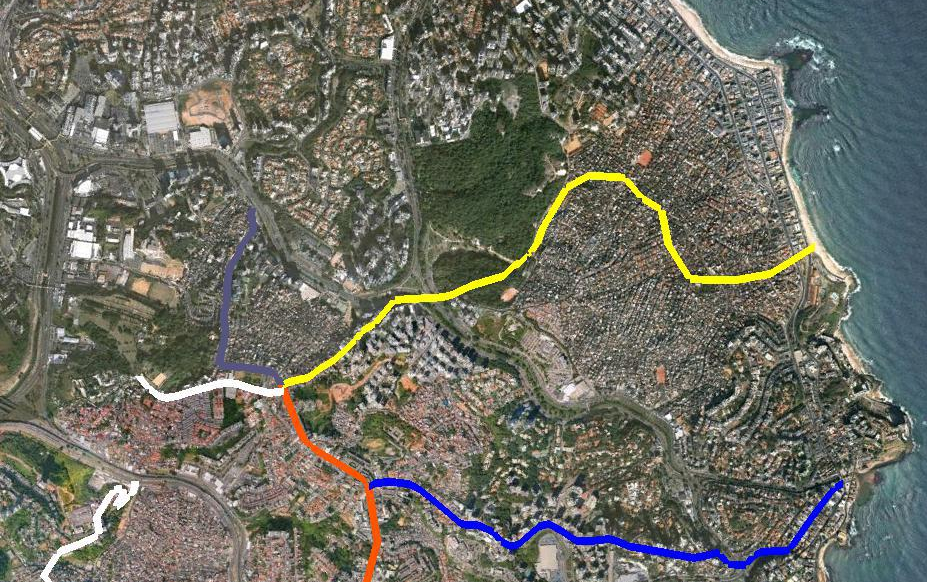
\includegraphics[width=0.7\textwidth]{3-cap2/complementos/mapas/armacaodalagoa-hoje.eps} 
\label{fig:armacaodalagoa-hoje}
}
\caption{Duas representações cartográficas do território correspondente às fazendas Alagoa, Amaralina, Santa Cruz, Ubarana e Pituba. Não foi possível avançar além do que o mapa mais antigo permitiu. \textbf{Fonte:} \citeonline{weyll_mappa_1851} e Google Earth.}
\end{figure}

A história fundiária destas cinco fazendas é inseparável, indissolúvel, indivisível. Limítrofes, integrantes do antigo morgado da Foz, seus antigos terrenos constituem, somados, a maior parte, quando não a totalidade, dos atuais bairros de Amaralina, Pituba, Nordeste de Amaralina, Santa Cruz, Rio Vermelho, Itaigara, Iguatemi, Chapada do Rio Vermelho e Vale das Pedrinhas.

Um dos grandes imóveis saídos do morgado da Foz foi a \textit{fazenda Alagoa}, localizada onde hoje estão os bairros do Rio Vermelho e Amaralina.

Quando ainda integrava o morgado foram construídos dentro dela, em 1768, um tanque de captação de água, um engenho (há muito desaparecido) e uma ermida \cite[p.~118]{campos_alagoa_1942}. A ermida, transformada em capela dedicada a Nossa Senhora dos Mares, ainda existe nos dias de hoje, incorporada ao Quartel de Amaralina, localizado no mesmo sítio onde se erguia a casa-grande do engenho.

Já desmembrada do morgado, a fazenda Alagoa foi adquirida em 1797 por Alexandre Teotônio de Sousa, tenente-coronel de granadeiros da guarnição de Salvador; alguns seus herdeiros remotos venderam-na em 1854 a José Álvares do Amaral\footnote{O primeiro sobrenome desta personagem histórica encontra-se grafado como ``Alves'' ou ``Álvares'' a depender da fonte. Foi mantida a grafia tal como foi encontrada.} \cite[p.~118]{campos_alagoa_1942}, com os seguintes limites constantes do \textbf{Livro Eclesial de Registro de Terras da Freguesia de Brotas}:

\begin{citacao}
Terreno de José Alves do Amaral

Em obediência ao despacho do senhor Vice-Presidente Missias de Leão, de 29 de abril de 1859, exarei o seguinte registro:

José Alves do Amaral, tendo o domínio útil da fazenda ``Alagôa'', situada nesta freguesia das Brotas, vem apresentala ao registro das terras. Principia o limite da dita fazenda, do lado da Ubarana, de propriedade útil do Major Manoel de Barros Paim, por um marco de pedra de cantaria collocado em mil setecentos e oitenta e nove na costa do mar em direção NO 35gº no qual se acha gravada a seguinte inscripção '1789', e partindo dahi no rumo que mostra o dito marco a encontrar a valla mestra divisória que passa nos fundos da dita fazenda Ubarana, e seguindo pela dita valla a encontrar a área nativa que limita com a fazenda ``Pituba'', de propriedade do Visconde do Rio Vermelho, e acompanhando a dita cerca até encontrar a estrada que conduz para a Cruz da Redempção em Brotas, dividindo sempre por esta estrada com a fazenda ``Santa Cruz'', de propriedade de Antonio Joaquim da Silva e Abreu, até o lugar chamado ``tanque'', e seguindo dahi pela valla mestra a desembocar no rio Camorogipe, e por este abaixo até sua foz no mar pela parte da Mariquita, confrontando por este lado com terras pertencentes ao Mosteiro de São Bento, tendo a dita fazenda toda a frente para o mar, pela costa as terras da dita fazenda [\textit{ilegível}] do senhorio direto Thomas da Silva Paranhos. Cumpre declarar que os limites da mencionada fazenda se encontram em litígio com os [\textit{ilegível}] confrontantes da Ubarana e Santa Cruz. Bahia, quatro de abril de mil oitocentos e cincoenta e nove. José Álvares do Amaral.

E nada mais continhão as declarações que me foram transmitidas. Brotas da Bahia, 3 de maio de 1859.

Vigº Ernesto de Olivª Valle\footnote{\textbf{BR BAAPB}, fundo Colonial, série Registros de Terra, livro 4675, f. 36 verso e 37.}
\end{citacao}

No mapa de \citeonline{weyll_mappa_1851} (cf. \autoref{fig:armacaodalagoa-1851}) há a indicação de uma ``Armação da Lagoa'', compatível com os relatos da existência de uma armação de pesca nesta fazenda desde os idos do século XVIII \cite[p.~120-121]{campos_alagoa_1942}. O mesmo mapa mostra uma estrada que a liga ao Largo de Brotas. Se seguirmos seu trajeto desde este largo até o mar e o compararmos com o trajeto de ruas atuais (cf. \autoref{fig:armacaodalagoa-hoje}), é plausível conceber alguns possíveis caminhos remanescentes desta antiga estrada\footnote{Com a base documental pesquisada até o momento é impossível descrever precisa e minuciosamente as ruas remanescentes desta estrada, e é possível mesmo que tal descrição documental sequer exista; a reconstituição desta estrada exigiria uma pesquisa \textit{in loco} com antigos moradores da Santa Cruz e do Nordeste de Amaralina para tentar recompor alguns traços perdidos desta estrada, profundamente modificada pela ocupação popular do território destes bairros, pelos loteamentos resultantes nos bairros de Amaralina e Pituba, e pela construção da avenida Juracy Magalhães e do Parque da Cidade.}

\begin{itemize}
\item Os dois caminhos saem do largo da Cruz da Redenção, descendo sua ladeira até o leito do rio Camorogipe, e o atravessam por meio de uma ponte (atualmente inexistente);
\item Uma primeira hipótese para um traçado remanescente desta estrada segue pela rua Onze de Novembro, ou Estrada da Santa Cruz, e daí pela rua do Futuro e pela avenida Nova República;
\item Uma segunda hipótese para o traçado corta caminho desde o leito do Camorogipe por dentro do atual Parque da Cidade, encontrando a avenida Nova República;
\item Da avenida Nova República o traçado segue encontrando-se com a rua Victorio Rossi para continuar pelo Beco da Cultura;
\item Uma linha imaginária ligaria o Beco da Cultura à rua Reinaldo de Matos, encontrando-se com a rua Cristóvão Ferreira;
\item Outra forma de ligar a avenida Nova República com a rua Cristóvão Ferreira seria sair da avenida para a rua Nova República, daí para a rua Valdomiro, depois para a travessa 20 de Junho, daí para as ruas do Areal e Ipanema, pela ruas Onze de Novembro e Francisco Sales até a rua dos Posseiros, e daí por uma linha imaginária até a rua Alto do Capim e, enfim, a rua Cristóvão Ferreira;
\item O caminho terminaria, por fim, na atual rua do Norte, ligada ao litoral por uma linha imaginária. 
\end{itemize}

É desta fazenda que deriva o loteamento, de final do século XIX, chamado \textit{Cidade Balneária Amaralina}, a ser detalhado no capítulo seguinte.

A compra da fazenda Alagoa foi fortemente contestada durante quase quarenta anos por Tomás da Silva Paranhos, comprador, como visto, do que restara do morgado da Foz \cite[p.~118]{campos_alagoa_1942}. Terminada a querela, diz um memorialista célebre que a fazenda teria sido rebatizada em 1912 como fazenda \textit{Amaralina} \cite[p.~118]{campos_alagoa_1942}; como se verá no capítulo seguinte, a documentação consultada durante esta pesquisa dá a entender que já na década de 1890 havia duas fazendas distintas, a \textit{Alagoa} e a \textit{Amaralina}.

Menos célebre que a fazenda Alagoa, a \textit{fazenda Santa Cruz} é assim descrita no \textbf{Livro Eclesial de Registro de Terras da Freguesia de Brotas}:

\begin{citacao}
Fazenda de Antonio Joaquim da Silva e Abreu

Antonio Joaquim da Silva e Abreu possue na freguesia de Nossa Senhora de Brotas da Capital da Bahia uma fazenda denominada ``Santa Cruz'', em terrenos proprios, aqual limita-se pelo nascente com a fazenda Ubarana, pelo poente com o rio Camorogipe, pelo norte com a fazenda Pituba e pelo sul com o mesmo rio Camorogipe na povoação da Mariquita. Bahia e Freguesia de Brotas, vinte e sete de novembro de mil oitocentos e cincoenta e oito. Antonio Joaquim da Silva e Abreu.

E nada mais continhão as declarações que me foram transmitidas. Brotas da Bahia, 27 de novembro de 1858.

Vigº Ernesto de Olivª Valle\footnote{\textbf{BR BAAPB}, fundo Colonial, série Registros de Terra, livro 4675, f. 36 e 36 verso.}
\end{citacao}

Não foi possível encontrar quaisquer outras referências a esta fazenda na documentação pesquisada, mas no capítulo seguinte se verá como esta fazenda foi loteada ao final da Primeira República.

A \textit{fazenda Ubarana} é assim descrita no \textbf{Livro Eclesial de Registro de Terras da Freguesia de Brotas}, num registro que se encontra severamente atingido pela ação do tempo:

\begin{citacao}
A fazenda denominada Ubarana, sita na f[regue]sia de N[oss]a Senhora de [Bro]tas, da Capital [da] Bahia, divide-se pelos la[do]s do Sul com a[s fa]zendas Alagôa e Santa Cruz, a saber [ilegível]dindo do [ilegível] da Ubarana do lado do Sul em [li]nha recta a Pedra da Marca pelo caminh[o] que vae para Brotas, afindar-se no rio Camorogipe, a encontrar do lado norte com a [ilegível] nativa de antigas árvores que faz a [divi]za com a fazenda da Pituba, descendo athe vizinhanças do mar, [ilegível] desta os limites [ilegível] referida fazenda do [ilegível] [ilegível]. Brotas, vinte e oito de novembro de mil oitocentos e cincoenta e nove. Manuel [ilegível] de Barros Paim.

E nada mais continhão as declarações que me foram transmitidas. Brotas da Bahia, 15 de janeiro de 1860.

Vigº Ernesto de Olivª Valle\footnote{\textbf{BR BAAPB}, fundo Colonial, série Registros de Terra, livro 4675, f. 40.}
\end{citacao}

Um resquício de memória desta fazenda ainda pode ser encontrado no nome da atual rua das Ubaranas, lindeira entre os bairros da Pituba e Amaralina, que corre paralela à avenida Manoel Dias da Silva entre as ruas Pará e Vandick Badaró.

Já a \textit{fazenda Pituba} tem seus limites assim descritos no \textbf{Livro Eclesial de Registro de Terras da Freguesia de Brotas}:

\begin{citacao}
Terras da Exmª Viscondessa do Rio Vermelho

Limites da legoa de terra que pertence a Excellentíssima Viscondessa do Rio Vermelho e o condomino seo filho Barão do Rio Vermelho. Na freguesia de Nossa Senhora das Brotas está a fazenda denominada Pituba em um [ilegível] de terras que pertenceu a Casa da Excellentíssima Marquesa de Niza, hoje ao Capitão Thomas da Silva Paranhos, e [ilegível] de posse por escriptura de foro perpetuo para a Excellentíssima Viscondessa do Rio Vermelho e seu filho o Barão do Rio Vermelho. Tem por limites a dita fazenda ao sul divide com a fazenda Ubarana, ao norte com terras do Engenho Santo Antônio, ao nordeste com terras de São Bento, onde está a Armação do Gregório, e a leste com o mar. Bahia, quinze de julho de mil oitocentos e cincoenta e nove. Barão do Rio Vermelho.

E nada mais continhão as declarações que me foram transmitidas. Brotas da Bahia, 15 de julho de 1859.

Vigº Ernesto de Olivª Valle\footnote{\textbf{BR BAAPB}, fundo Colonial, série Registros de Terra, livro 4675, f. 38.}
\end{citacao}

Como se pode inferir dos limites constantes nos registros de terra, a povoação da Mariquita era o ponto de convergência, e portanto de conflito, entre os limites das fazendas Santa Cruz e Alagoa. A deterioração do registro da fazenda Ubarana dificulta compreender os limites entre ela e as demais fazendas, pois a descrição de alguns marcos foi corroída pela tinta.



\subsection{Campinas e as terras dos Ladislau}

\begin{figure}[!htp]
\centering
\subfloat[Em 1851]{
\includegraphics[width=0.7\textwidth]{3-cap2/complementos/mapas/campinas-1851.eps} 
\label{fig:campinas-1851}
}
\  %espaco separador
\subfloat[Atualmente]{
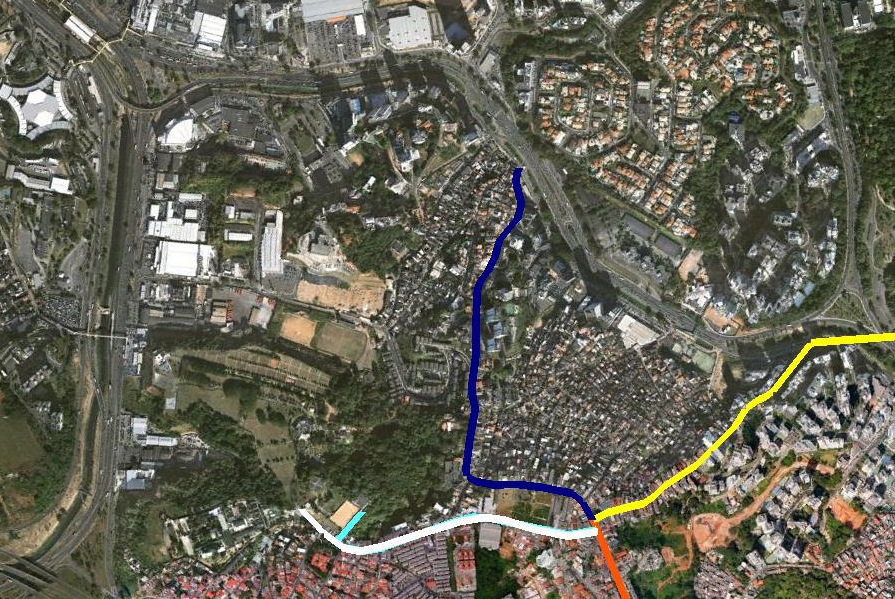
\includegraphics[width=0.7\textwidth]{3-cap2/complementos/mapas/campinas-hoje.eps} 
\label{fig:campinas-hoje}
}
\caption{Duas representações cartográficas do território correspondente às terras dos Ladislau. \textbf{Fonte:} \citeonline{weyll_mappa_1851} e Google Earth.}
\end{figure}

Toda a área que hoje conhecemos como \textit{Campinas de Brotas} era, no século XIX, de propriedade de integrantes da família \textit{Ladislau}, cujo patriarca, João Ladislau de Figueredo e Melo, vinha a ser sogro do mesmo José Álvares do Amaral reivindicante da fazenda Alagôa. O próprio nome da área -- Campinas -- deriva de duas das herdades da família.

A primeira delas era a fazenda Campina Grande:

\begin{citacao}
Fazenda Campina Grande

Rosa Ladislau de Figueredo e Melo e Virgínia Ladislau de Figueredo e Melo possuem em condomínio nesta Freguesia de Nossa Senhora das Brotas uma Fazenda denominada Campina Grande, em que há Engenho de fabricar assucar, e que comprehende a fazenda do mesmo nome Campina Grande, [ilegível] Carregado e Chacôco, terras proprias, que de [ilegível] [ilegível] um lado com a roça da dita Rosa Ladislau de Figueredo e Melo no lugar da Cruz da Redempção e com outra denominada Campina Pequena de dona Michelina Ladislau e Silva e dona Joanna Fausta Ladislau e Silva, de outro com terras do Matatu de José Antonio Pinto pelo riacho de mesmo nome, e mais com terras do Girão de Joaquim Caetano de Almeida Couto, ou quem mais direito for, pelo riacho Camorogipe, outra com terras que forão de dona Maria de Argôlo, e com as do Engenho Santo Antônio da Viscondessa do Rio Vermelho e sua filha dona Judith Constança da Cunha, pelo dito Camorogipe, e pelo outro com a estrada que sobe da ponte do mesmo Camorogipe e com terras que forão de João Paulo e seu irmão Fabião. Esta declaração vae por uma de nós feita e por ambas assignada. Bahia e Freguesia de Nossa Senhora das Brotas, primeiro de junho de mil oitocentos e cincoenta e oito. Rosa Ladislau de Figueredo e Melo, Virgínia Ladislau de Figueredo e Melo.

E nada mais continhão as declarações que me foram enviadas. Brotas da Bª, 5 de junho de 1858.

Vigº Ernesto de Olivª Valle\footnote{\textbf{BR BAAPB}, fundo Colonial, série Registros de Terra, livro 4675, f. 4 verso e 5.}
\end{citacao}

A outra, a fazenda Campina Pequena:

\begin{citacao}
Roça Campina Pequena

Michelina Ladislau e Silva e Joanna Fausta Ladislau e Silva possuem nesta Freguesia de Nossa Senhora das Brotas uma roça denominada Campina Pequena com casa de vivenda e outras benfeitorias, terras próprias, e que se divide pela frente com terras de Raphael e José Joaquim, e por outro lado com a Quinta das Beatas pelo riacho que a separa, por outro com a estrada que entra para o Engenho da Campina Grande, e pelo fundo com terras do mesmo Engenho. Esta declaração vae feita por uma de nós e por ambas assignada. Bahia e Freguesia de Nossa Senhora das Brotas, primeiro de junho de mil oitocentos e cincoenta e oito. Michelina Ladislau e Silva, Joanna Fausta Ladislau e Silva.

E nada mais continhão as declarações que me forão enviadas. Brotas da Bahia, 4 de junho de 1858.

Vigº Ernesto de Olivª Valle\footnote{\textbf{BR BAAPB}, fundo Colonial, série Registros de Terra, livro 4675, f. 5 e 5 verso.}
\end{citacao}

No mapa de \citeonline{weyll_mappa_1851} (cf. \autoref{fig:campinas-1851}), vê-se nitidamente que o ``Engº'' marcado perto de ``Prambeé'' corresponde muito proximamente à descrição documental do Engenho Campina Grande, situado na baixada hoje correspondente à rua Santiago de Compostela. No cume logo abaixo do ``Engº'' no mapa, onde hoje se situam  o cemitério Jardim da Saudade e o Abrigo Salvador, tem início uma estrada que corresponde à atual rua Campinas de Brotas. À atual rua Teixeira Barros corresponde a antiga Estrada do Beijú; se o mapa de Weyll continuasse mais ao leste, seria possível observar como esta estrada se unia à Estrada das Armações no trecho onde se cruzam, hoje, as avenidas Paulo VI e Antônio Carlos Magalhães. 

Em 1845 se anunciava a venda, no Campina Grande, ``distante desta cidade tres quartos de legoa'', de ``capim bom e verde, já cortado, a 120 a arroba''\footnote{\textbf{O Mercantil}, 27 set. 1845, p. 4.}. Notícia de prisão efetuada em suas matas indica que o engenho Campina ainda existia enquanto tal em 1881\footnote{\textbf{O Monitor}, 10 jun. 1881, p. 1.}.





\subsection{A Estrada de Brotas e seus arredores}

\begin{figure}[!htp]
\centering
\subfloat[Em 1851]{
\includegraphics[width=0.4\textwidth]{3-cap2/complementos/mapas/estbrotas-1851.eps} 
\label{fig:estbrotas-1851}
}
\  %espaco separador
\subfloat[Atualmente]{
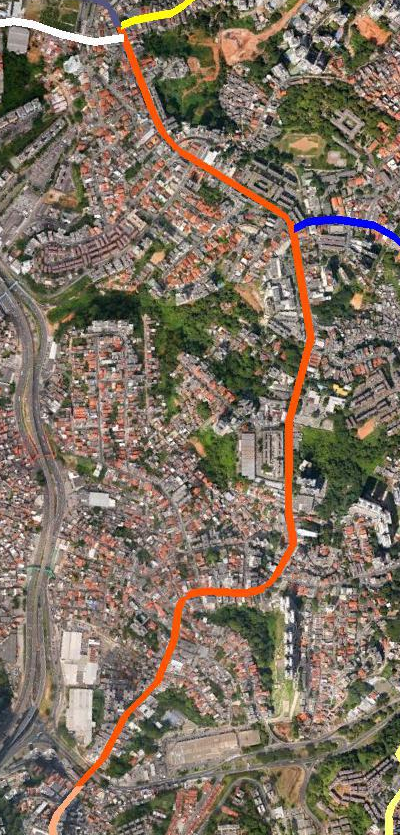
\includegraphics[width=0.4\textwidth]{3-cap2/complementos/mapas/estbrotas-hoje.eps} 
\label{fig:estbrotas-hoje}
}
\caption{Duas representações cartográficas do território correspondente à Estrada de Brotas (atual av. D. João VI). \textbf{Fonte:} \citeonline{weyll_mappa_1851} e Google Earth.}
\end{figure}

No século XVIII saía do Portão da Piedade uma estrada então conhecida como \textit{Caminho Grande}, correspondente ao que veio depois ser a \textit{Estrada de Brotas}, atual Avenida D. João VI; era por aí que se partia da cidade ao Rio Vermelho, passando pelo paço do Acupe, integrante do morgado da Casa da Torre \cite[p.~85]{campos_brotas_1942}. Patente de sargento-mor da freguesia de ``Nossa Senhora de Brotas do Caminho Grande'' concedida a Veríssimo de Campos de Carvalho em 1725 \cite[p.~114]{texmel_manusbn_1896} mostra como era conhecida a freguesia em seus primórdios.

Infelizmente não foi possível encontrar registros seguros do traçado completo do Caminho Grande, exceto por uma referência que o qualificou como `perigoso'' e disse passar ele ``pela Lapa e atual Campo da Pólvora, pela crista dos montes e pelos divisores de águas, passando em Fonte Nova e por Brotas até aquele ponto da costa oceânica'' \cite[p.~488]{sampaio_salvador_2016}. Com base no mapa de \citeonline{weyll_mappa_1851} (cf. \autoref{fig:estbrotas-1851}), pode-se conjecturar, entretanto, que a ligação entre a Piedade e o atual Largo do Paranhos, onde tinha início a Estrada de Brotas, fosse feita pelo trecho da atual avenida Joana Angélica que vai até a ladeira da Fonte Nova e por esta própria ladeira, chegando, através da atual ladeira dos Galés, até o referido largo, completando assim o primeiro trecho. Daí em diante, pode-se apenas conjecturar, inconclusivamente, por onde o Caminho Grande desceria rumo ao Rio Vermelho.

O jornal quinzenal \textbf{A Lei}, num breve perfil biografico, indicou que em 1848 o brigadeiro Evaristo Ladislau e Silva ``concorreu para o melhoramento da estrada de Brotas''\footnote{\textbf{A Lei}, ano 2, nº 2, fev. 1877, pp. 2-3.}; certamente terá a ver com o fato de que entre 1848 e 1849 a presidência da província investiu 2:269\$344 na Estrada de Brotas, comprometendo-se a investir outros 5:000\$000 em melhoramentos na via; investiu também 1:414\$000 no encanamento do rio Camorogipe, empenhando-se a investir outros 177:539\$000 na mesma finalidade \cite{bahia_rpe_1849}.

Como a Estrada de Brotas era -- e continua sendo, se somarmos as atuais ruas que estão sobre seu antigo leito -- muito comprida, é preciso fazer como os da época e subdividi-la em alguns pontos notáveis e cercanias.

O primeiro deles é o \textit{Largo de Brotas}, existente desde a fundação da igreja matriz. Em 1882 uma casa posta a leilão nesta localidade foi assim descrita e avaliada:

\begin{citacao}
...uma casa ao largo da matriz de Brotas, n. 14, com 5 metros e 46 centimetros de frente, que é dobrada e de azulejos, com porta e 2 janellas, sala feichada, 3 quartos, sala de jantar, cosinha, quintal e sotão, em terreno proprio [\dots]\footnote{\textbf{Diário da Bahia}, 30 set. 1882, p. 3.}.
\end{citacao}

Apesar de um célebre memorialista afirmar que o \textit{largo da Cruz da Redenção}, até hoje existente, foi mandado abrir em 1841 na Estrada de Brotas pelo coronel João Ladislau de Figueredo e Mello, dono do engenho Campinas \cite[p.~88]{campos_brotas_1942}, já se encontra anúncios de venda de roça na mesma localidade em 1838\footnote{\textbf{Correio Mercantil}, vol. 3, nº 583, 19 out. 1838, p. 4.}.

Em 1882 uma casa posta a leilão nesta localidade foi assim descrita e avaliada:

\begin{citacao}
Uma casa situada à rua da Redempção, freguezia de Brotas, com 3 metros e 30 centimetros de frente, e n'esta uma porta e janella, sala, dous quartos, sala de jantar em commum com a cosinha, pequeno quintal; divide-se por um lado com casa do intestado e pelo outro com Luiz Mendes, avaliada por 100\$000\footnote{\textbf{Diário da Bahia}, 3 jan. 1889, p. 2.}.
\end{citacao}



Caetano Vicente de Almeida Galião, juiz de paz do segundo distrito da Sé em 1835, possuía um pequeno engenho e uma pequena fazenda em Brotas \cite[p.~239]{REIS2004males}.

\subsubsection{Cruz das Almas}

Já em 1870, um certo Miguel dos Santos Prates vinha a público agradecer aos que acompanharam o cortejo fúnebre de seu pai desde sua casa, na Estrada da Cruz das Almas, até o cemitério de Brotas\footnote{\textbf{O Monitor}, 20 jun. 1870, p. 3}

\subsubsection{Cemitério de Brotas}

Em 1871 o cemitério da freguesia de Brotas já demandava ser alargado\footnote{\textbf{Jornal da Bahia}, ano XIX, nº 5.446, 22 set. 1871, p. 1}, e em 4 de julho de 1876 o juiz e mesário da irmandade do Santíssimo Sacramento de Nossa Senhora de Brotas requereu ao administrador do cemitério 30 metros quadrados de terreno devoluto para a construção de carneiros para a irmandade\footnote{\textbf{O Monitor}, 16 jul. 1876, p. 2}. Em 1879 a presidência da província transferiu a administração do cemitério para a Câmara Municipal por meio da lei 1.943, de 26 de agosto do mesmo ano\footnote{\textbf{O Monitor}, 30 ago. 1879, p. 1.}.

\subsubsection{Estrada e Alto do Beijú}


\subsection{A fazenda Boa Vista e seus arredores}

\begin{figure}[!htp]
\centering
\subfloat[Em 1851]{
\includegraphics[width=\textwidth]{3-cap2/complementos/mapas/boavista-sangradouro-1851.eps} 
\label{fig:boavista-sangradouro-1851}
}
\  %espaco separador
\subfloat[Atualmente]{
\includegraphics[width=\textwidth]{3-cap2/complementos/mapas/boavista-sangradouro-hoje.eps} 
\label{fig:boavista-sangradouro-hoje}
}
\caption{Duas representações cartográficas do território correspondente à fazenda Boa Vista (atual Engenho Velho de Brotas) e ao Sangradouro (atual Santo Agostinho). \textbf{Fonte:} \citeonline{weyll_mappa_1851} e Google Earth.}
\end{figure}

O mapa de \citeonline{weyll_mappa_1851} mostra ainda uma longa estrada saindo das terras da Boa Vista em direção a uma estrada que corresponde à atual avenida Cardeal da Silva. Remanescentes desta estrada são as ruas Almirante Alves Câmara e Padre Luiz Figueira, no Engenho Velho de Brotas, e Sérgio de Carvalho, no Vale da Muriçoca; mais ou menos no ponto onde a Sérgio de Carvalho faz esquina com a atual av. Edite, também no Vale da Muriçoca, o mapa de Weyll indica uma ponte sobre um riacho, e daí em diante a estrada seguia um curso hoje inexistente, que terminava aproximadamente na altura da atual Ladeira das Carmelitas, na Federação. Seria esta a Estrada da Boa Vista, estendendo-se desde o Largo dos Paranhos até a atual Cardeal da Silva?

\subsubsection{Moinho}



\subsubsection{Capela do Deus Menino}



\subsubsection{Dique Pequeno}



\subsubsection{Monte de Belém}



\subsubsection{Porto dos Saveiros}



\subsubsection{Estrada da União}



\subsection{A Estrada Dois de Julho}

\begin{figure}[!htp]
\centering
\subfloat[Em 1851]{
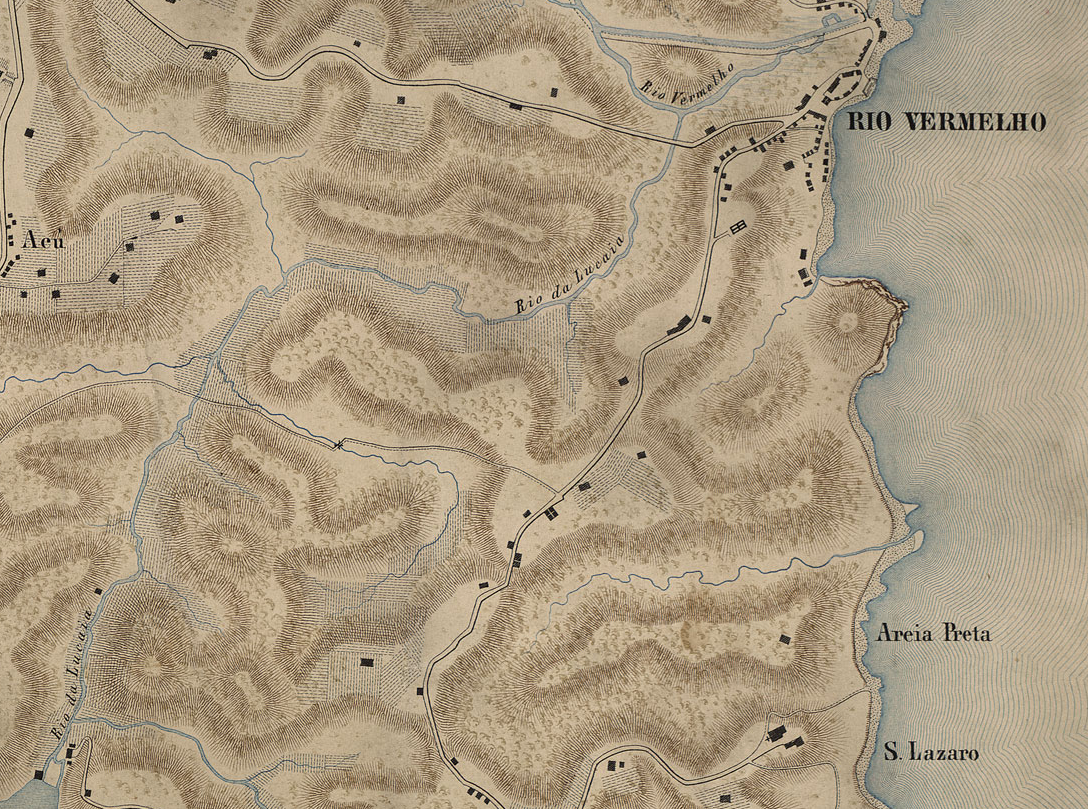
\includegraphics[width=0.7\textwidth]{3-cap2/complementos/mapas/e2j-1851.eps} 
\label{fig:e2j-1851}
}
\  %espaco separador
\subfloat[Atualmente]{
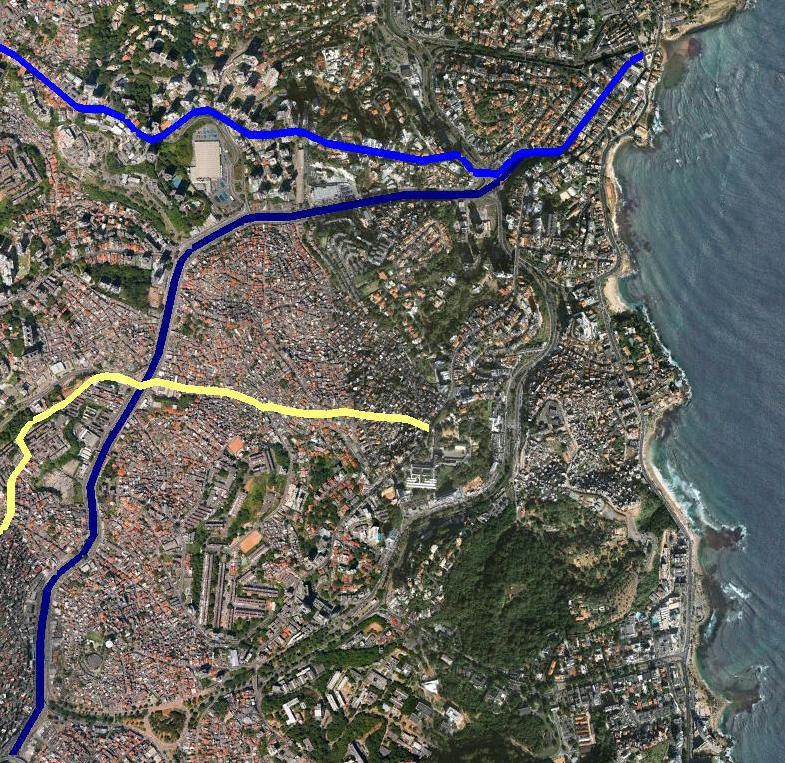
\includegraphics[width=0.7\textwidth]{3-cap2/complementos/mapas/e2j-hoje.eps} 
\label{fig:e2j-hoje}
}
\caption{Duas representações cartográficas da Estrada Dois de Julho (atual av. Vasco da Gama). Em 1851 ela não estava construída, mas corresponde ao leito do rio Lucaia. \textbf{Fonte:} \citeonline{weyll_mappa_1851} e Google Earth.}
\end{figure}

Em 10 de maio de 1879 o presidente da província ordenou ao diretor de obras públicas 

\begin{citacao}
\dots lavrar contracto n'essa repartição com o Commendador Giusto Ariani para o serviço de deseccação do terreno na estrada Dous de Julho, entre a fábrica de lapidação de diamantes pertencente aos negociantes Costa Pinto \& Filhos e a ladeira que segue para Brotas, e bem assim para a canalisação da parte do riacho Lucaia entre aquelles dous pontos\footnote{\textbf{O Monitor}, 3 jun. 1879, p. 1.}.
\end{citacao}
\subsection{O Matatu Grande, o Matatu Pequeno, Quinta das Beatas e arredores}\label{subsec:matatubeatas}

Em 17 de junho de 1799 o Conselho Ultramarino deu parecer favorável a requerimento de porte de armas defensivas feito pelo capitão Pedro Gomes Ferreira; o militar residia ``na sua fazenda do Matatu'' \cite[p.~228]{castralmeida_ultramar_1914}, indicando que já no século XVIII a área era reconhecida por este nome. 

Há duas versões para a etimologia do topônimo. A primeira e mais conhecida diz ser ele de origem tupi, significando ``mata escura'', ``floresta negra'' \cite[p.~281]{sampaio_tupi_1987}. A segunda, menos conhecida, diz que se trata de um africanismo de origem bantu, significando ``lugar deserto, isolado'' \cite[p. 46]{dorea_ruas_2006}. Qualquer das duas versões, seja pela existência de mata fechada, seja escassez populacional, passam a impressão de um lugar distante, ermo, pouco povoado, e é bem possível que assim o fosse no século XVIII quando encontramos a primeira referência ao nome; no século XIX, entretanto, o \textbf{Livro Eclesial de Registro de Terras da Freguesia de Brotas} indica a existência de muitos pequenos proprietários de terras na área, sendo ela a que mais tem registros fundiários em toda a freguesia\footnote{\textbf{BR BAAPB}, fundo Colonial, série Registros de Terra, livro 4675.}.

No mapa de \citeonline{weyll_mappa_1851}, lido no sentido NNE-SSE (cf. \autoref{fig:matatu-1851}), a área é representada por três cumeadas. 

\begin{figure}[!htp]
\centering
\subfloat[Em 1851]{
\includegraphics[width=0.7\textwidth]{3-cap2/complementos/mapas/matatu-1851.eps} 
\label{fig:matatu-1851}
}
\  %espaco separador
\subfloat[Atualmente]{
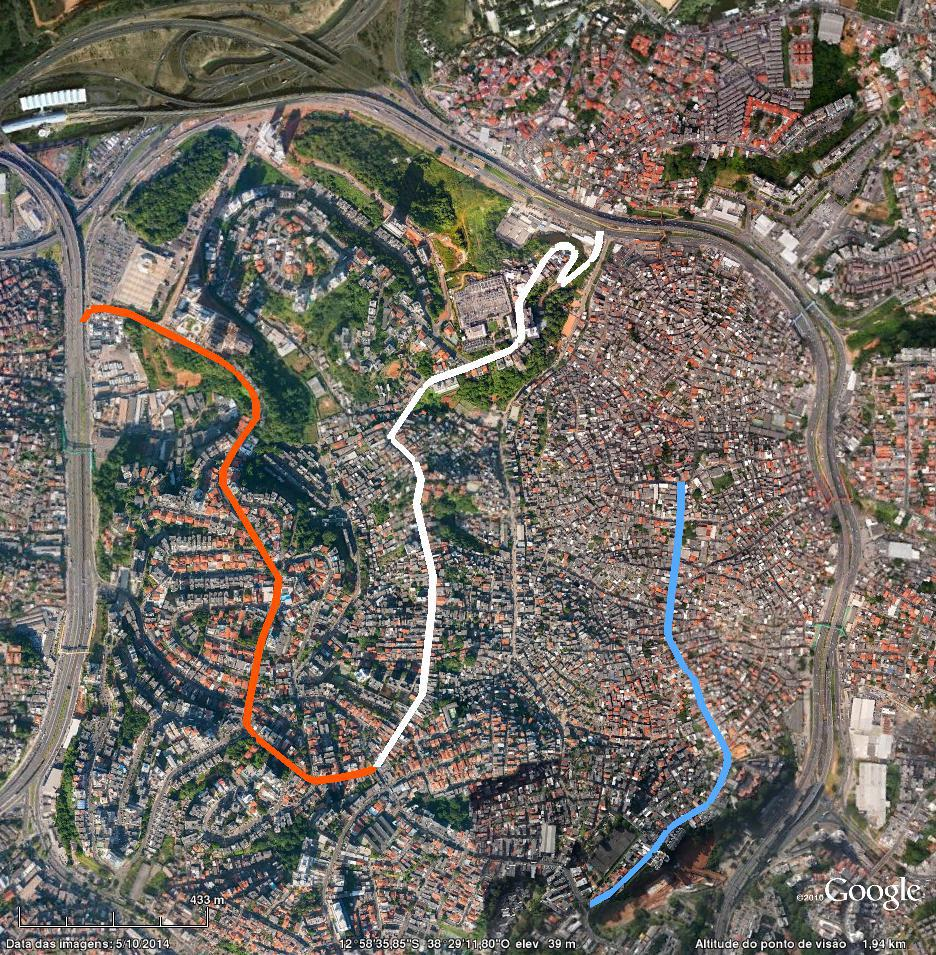
\includegraphics[width=0.7\textwidth]{3-cap2/complementos/mapas/matatu-hoje.eps} 
\label{fig:matatu-hoje}
}
\caption{Duas representações cartográficas do Matatu, mostrando a rua da Valla (atual av. Heitor Dias), a Estrada da Pólvora (atual rua Raul Leite), a Estrada do Matatu Grande (atual rua Luiz Anselmo) e a Quinta das Beatas (atual Cosme de Farias). \textbf{Fonte:} \citeonline{weyll_mappa_1851} e Google Earth.}
\end{figure}

 A terceira tem uma estrada, correspondente à atual rua Cosme de Farias, que vai dar na ``Quinta das Biatas''
 
 . No mesmo mapa é possível encontrar símbolos indicativos de construções pontilhando a cumeada do Matatu Grande, embora a cumeada onde se localiza a Casa da Pólvora apresente-se pouco povoada, assim como a da Quinta das Beatas.

Novamente lendo o mapa de Weyll no sentido NNE-SSE (\autoref{fig:matatu-1851}), quatro rios escavam os vales circundantes destas cumeadas. Temos em primeiro lugar o \textit{rio das Tripas}, afluente do Camaragipe, vizinho ao qual corria a rua da Vala, no trecho correspondente à atual avenida Heitor Dias. O segundo rio é indicado por Weyll como sendo o \textit{Santo Antônio}, hoje um esgoto \cite[p.~136]{santos_aguas_2010} que corre quase paralelamente à atual rua do Baixão. O terceiro rio é o \textit{Córrego das Beatas} \cite[p.~158]{santos_aguas_2010}, correspondente, grosso modo, à atual Baixa do Matatu, também transformado em esgoto. O Córrego das Beatas é afluente do rio \textit{Bonocô}, que no mapa de \citeonline{weyll_mappa_1851} separa a Quinta das Beatas da cumeada cortada pela Estrada de Brotas.

Dado o grande tamanho da área analisada, será preciso subdividi-la nos pontos notáveis e nomes pelos quais era conhecida na época, atualizando-os quando necessário.

A porta de entrada para o Matatu, no sentido de quem vem da Ladeira dos Galés, é o \textit{largo do Paranhos}, assim batizado em homenagem ao já mencionado latifundiário Tomás da Silva Paranhos.

Em 1879 foi anunciado o leiloamento de uma roça de propriedade de Herman e Sophia Both, penhorada pela Sociedade de Commercio, localizada no largo do Paranhos, descrita no anúncio a seguir. bserve-se com detalhe a estrutura e o valor do imóvel à venda; trata-se de fazenda bem constituída, de gente abastada o suficiente para ter inquilinos:

\begin{citacao}
Uma roça em terreno proprio, na freguezia de Brotas, largo denominado de Paranhos, tendo a frente para o mesmo largo, dividindo-se pelo lado direito com a roça que foi do Bacharel Firmino Duarte Gameleira; pelo esquerdo, com a estrada que vai para a Quinta das Beatas; e pelo lado direito continuando de fundo à frente com terreno que foi do dito Bacharel Gameleira onde vae acabar. Medida a frente da roça, acha-se n'ella 336m 10c; do canto que vira para a estrada da Quinta das Beatas até encostar na roça que foi do Bacharel Gameleira, havendo n'este lado 143m 60c; de terreno, com o fundo de 43m 25c, que foram dados por aforamento a diversos, pelos executados, de modo que fica a frente propriamente dita da roça com 180m 50c, desde o terreno aforado até a esquina para a estrada das Boiadas, e essa frente está fechada por muros de boa construcção, tendo um portão de ferro por onde é a entrada principal para a roça e casa de morada. A entrada do portão para a casa é guarnecida de perfeitas cercas de pitangueiras, que terminam em 2 carramanchões sobre pilastras de pedra de cantaria; dentro das cercas de pitangueiras existem diversas arvores, como saputizeiros, abacateiros, laranjeiras etc., havendo no lado esquerdo da mesma roça diversas divisões formadas por cercas de pitangueiras, e em todos esses lotes diversas arvores, como as declaradas, cuja quantidade é a seguinte:

Na parte cultivada da roça existem: 60 jaqueiras, 73 mangueiras, 193 laranjeiras, 10 pes de fructa pão, 8 cajazeiras, 8 abacateiros, 24 saputizeiros, 23 coqueiros, 2 genipapeiros, 1 tamarindeiro, 4 [ilegível] de parreira, sendo algumas de pés direitos de cantaria, 1 brejo que termina em uma ribanceira, onde existe uma capoeira para corte de madeira, 1 telheiro fechado por paredes de taboas com uma machina à vapor em bom estado, serve para conduzir agua a um deposito junto á propriedade da morada, a qual agua é puxada por um encanamento de ferro, de um deposito de pedra e cal cimentado e coberto tambem com telheiro, 1 banheiro fechado por paredes de pedra e cal, e coberto de telhas, com 2 portas e 3 torneiras de bronze.

Uma casa de campo de gosto antigo com varandas fechadas por frontoes, e n'elles peitoris, tendo no lado direito da varanda, 1 oratorio de celebrar missa. A entrada é por uma porta entre 4 janelas, com sala aberta que occupa a porta e 2 janelas, e 1 gabinete em cada lado, tendo cada gabinete 1 janella, e a entrada para o interior da casa é pela sala de jantar que dá em 1 salão, havendo de cada lado deste 1 corredor, com diversos repartimentos que são: 10 quartos, dispensa e cozinha, toda construida de pedra e cal e de gosto antigo. Depois desses repartimentos um grande salão de pedra e cal, com paredes dobradas, feito muito depois da casa, e de gosto moderno, rodeado de janellas de vidraças, isto é, com janelas de vidraças no fundo e no lado, e a parte por onde abre-se para um terraço d'onde desce-se para o centro da roça por uma escada de pedra, sobre este salão há um sotão para onde sobe-se por uma escada interna, tendo o mesmo sotão 4 divisões eguaes (4 grandes quartos ou 4 pequenas salas) cada uma com 2 janelas de vidraças, pelo que é o dito sotão rodeado de janellas, tanto a sala da frente como os quartos e o salão são forrados; a sala e os mais commodos terreos são cimentados, e o sotão é de lages de pedra; a casa descripta e o seu acrescimo (salão e sotão) tem de frente 12m60c de comprimento de frente a fundo 38m30c, cinco senzalas cobertas de telha em estado de reparo, dentro da roça, com 25m90c de frente; e em seguimento as mesmas senzalas 2 cazinhas que estão alugadas, e cujos inquilinos aproveitam-se na entrada e sahida do porão da cocheira.

Em frente ás senzalas e encostado ao muro da roça, existe um grande armazem, onde foi antiga estribaria, que ainda hoje tem em parte mangedouras, armazem esse que é coberto de telhas e precisa de reparos. A roça, casa e mais dependencias as avaliaram em 10:000\$000 [\dots]\footnote{\textbf{O Monitor}, 10 dez. 1879, p. 2.}.
\end{citacao}

O.

Passado o largo do Paranhos, chega-se de imediato à estrada que os contemporâneos chamavam das \textit{Pitangueiras}, curto trecho entre o largo e a estrada do Matatu Pequeno, hoje conhecida como Rua Barros Falcão. 

A primeira notícia encontrada acerca da existência do ``povoado das Pitangueiras'' é de 1871, numa situação polêmica. Uma escola primária masculina havia sido recentemente removida para este povoado, medida elogiada pelo rápido crescimento das turmas e pela abertura de turmas noturnas para artistas-operários\footnote{\textbf{Jornal da Bahia}, ano XIX, nº 5.445, 21 set. 1871, p. 1.}; tal remoção, entretanto, teria prejudicado os moradores do largo de Brotas, que só em 1876, depois de muito peticionar ao governo provincial, conseguiram deste a contratação de professores particulares para meninos e meninas da localidade\footnote{\textbf{O Monitor}, 3. set. 1876, p. 1.}. A situação, entretanto, ainda não havia melhorado em 1877, como se vê neste clamor assinado por um ``Amigo das Letras'':

\begin{citacao}
\textbf{Aos senhores deputados provinciaes}

Pedimos aos senhores deputados provinciaes que se dignem lançar suas vistas sobre a freguezia de Brotas desta capital, que muito necessita de duas escolas, sendo uma para cada sexo. As cadeiras dessa freguezia acham-se funcionando no logar denominado Pitangueiras -- de forma que um grande numero de crianças de um e outro sexo que moram no largo de Brotas e no Engenho Santo Antonio não podem receber a instrucção primaria.
Bahia, 18 de março de 1877\footnote{\textbf{O Monitor}, 22 mar. 1877, p. 3.}.
\end{citacao}

Ainda em abril de 1877 a situação da escola em Pitangueiras parecia periclitante, pois sua transferência para um extremo da freguesia resultara em grande evasão escolar\footnote{\textbf{O Monitor}, 28 abr. 1877, p. 1.},

Não é difícil deduzir desta situação que Pitangueiras era localidade de difícil acesso para os moradores do largo de Brotas e do Engenho Santo Antônio; pode-se igualmente deduzir a hipótese de que estas duas últimas localidades tivessem, entre 1871 e 1877, número de moradores maior que o de Pitangueiras. 

É certo, entretanto, que Pitangueiras concentrava razoável infraestrutura urbana, pois anúncio de casa a alugar nesta localidade em 1879 indicava ter a mesma ``os commodos necessarios para familia e encanamento de gaz''\footnote{\textbf{O Monitor}, 17 maio 1879, p. 2.}. Na mesma linha vai o anúncio de leiloamento dos seguintes imóveis, todos de bom padrão para a época:

\begin{citacao}
\textbf{Bens de raiz -- }Uma casa abarracada sita à rua das Pitangueiras, freguesia de Brotas, de n. 159, edificada em terreno proprio, com 8 metros e 10 centimetros de frente e 24 metros e 10 centimetros de fundo que dá para a rua Sete de Setembro, tendo de lado que dá para o beco 18 metros e 80 centimetros, com terraço na frente com gradil de ferro; a casa tem 2 janellas de peitoril e porta de vidraça no centro, 5 janellas do lado, sala de espera com porta para o becco, sala de visita, 2 quartos, salla de jantar e dispensa, e toda ella forrada, salla de gommar e cozinha, 3 quartos no quintal, lenheiro e sofás de cimento e concha para recreio, quintal todo murado com um portão para a dita rua, sotão com sala e 3 quartos, paredes todas dobradas, divide-se por um lado com casa do mesmo casal, avaliada por 4:000\$000.

Uma casa abarracada sita na dita rua e freguezia, de n. 157, edificada em terreno proprio, com 7 metros e 80 centimetros de frente com terraço e gradaria de ferro, com 2 janellas e porta no centro, sala de frente, 3 quartos, sala de jantar e toda ella forrada, dispensa, cozinha, sala de gommar com 2 quartos no quintal, sotão com janellas para a frente e fundo, com sala e 3 quartos, quintal todo murado com porteira para a rua Sete de Setembro, divide-se a casa por outro lado com casa do casal, avaliada por 3:000\$000.

Um terreno sito à rua Sete de Setembro, na dita freguezia, tendo de comprimento 38 metros, dividindo-se pelo fundo com terrenos do Hospital Militar, tendo diversas casas n'elle edificadas, avaliado cada metro por 15\$000 e todos por 570\$000 [\dots]\footnote{\textbf{O Monitor},3 out. 1879, p. 2.}.
\end{citacao}

Passado trecho da estrada das Pitangueiras, chega-se a uma esquina onde se abre a estrada que conduz à \textit{Quinta das Beatas}. A fazenda que ficou conhecida por este nome, no atual bairro de Cosme de Farias, tem sua descrição no \textbf{Livro Eclesial de Registro de Terras da Freguesia de Brotas} extremamente danificada pela ação do tempo:

\begin{citacao}
Quinta das Beatas

[ilegível] fazenda denominada Quinta das Beatas é propriedade do Recolhimento do Senhor Bom Jesus dos [Perd]oens, está situada na freguesia de Nossa Senhora  [de] Brotas, confina pelo nascente com a fazenda de[no]minada Campina, dos herdeiros do coronel João Ladis[la]u de Figueredo, e Matatu Grande, pertencente ao [ilegível] Pinto, pelo poente com a roça do tenente[-coron]el Pinheiro e com o capitão Paranhos, pelo sul [com] a roça de Amorim Vianna, com a Torre e com a [ilegível] e pelo norte com o Matatu pequeno e com [ilegível] [ilegível] Paranhos. Bahia, dezesseis de março de [mil oitocentos e] sessenta. Anna Maria Magdalena Re[jente]. 

[E nada mais] se continha em as ditas declarações [que me for]am enviadas.

Brotas da Bª, 20 de [março de 1860].

Vigº Ernesto de Olivª Valle\footnote{\textbf{BR BAAPB}, fundo Colonial, série Registros de Terra, livro 4675, f. 40 verso.}
\end{citacao}

A antiga sede da fazenda, a julgar pelo que mostra o mapa de \citeonline{weyll_mappa_1851}, estaria em algum lugar no trecho da atual rua Cosme de Farias situado entre as esquinas das atuais ruas Jaguarari e Lima Durval.

A relação entre o Recolhimento dos Perdões e a Quinta das Beatas é um dos mais acabados exemplos do \textit{rentismo}, sustentáculo econômico de tantas ordens religiosas católicas desde a fundação de Salvador até o presente. Na tentativa de fazer subir sua ordem na hierarquia eclesial (de \textit{recolhimento} a \textit{casa de professas}), mais especificamente como parte da ordem das carmelitas calçadas, as irmãs recolhidas nos Perdões argumentaram por todos os meios possíveis, incluindo os econômicos; em 1820 alegaram possuir, além do 

\begin{citacao}
recato e honestidade em que vivião, o possuirem renda sufficiente de 28 predios urbanos, a grande roça de nossa Sra. da Conceição das Brotas, mais conhecida por \textit{quinta das beatas}, não pequena porção de terreno arrendado e aforado, além de 16:000\$000 rs. em dinheiro de varios legados [\dots] \cite[p.~231]{accioli_memorias5_1937}.
\end{citacao}

Embora o relato apresente mais uma das tentativas frustradas de ascensão hierárquica das recolhidas, deixou evidente seu poder econômico. Pequeno, se comparado ao dos beneditinos, por exemplo \cite{bento_tombo_1945}, mas, mesmo assim, \textit{poder}.

Por ser de 1851, o mapa de Weyll ainda não poderia mostrar a \textit{Ladeira do Fabrício}, conhecida a princípio como \textit{Estrada do Sangradouro ao Matatu}, que corresponde ao trecho que inicia na Rua dos Tupys, esquina com a atual Rua do Sangradouro, e segue pela Ladeira dos Bandeirantes até encontrar-se com a estrada para o Matatu no local onde hoje a Ladeira dos Bandeirantes faz encruzilhada com as atuais ruas Alberto Torres, Barros Falcão e Amazonas. Esta ladeira foi mandada abrir em 1876 pelo governo provincial, em obras supervisionadas por uma comissão ``composta do Tenente-Coronel Fabricio Alves de Araujo, Bacharel Firmino Duarte Pacifico Gameleira e Negociante Manuel da Silva Pereira Guimarães'' \cite[p.~23]{bahia_1878}. A obra já se encontrava concluída no ano seguinte, sendo alargada de seus 8,8m originais para a largura de 11m e tendo recebido na mesma ocasião ``declives menos fortes'' \cite[p.~228]{bahia_1879}, e em 1885 recebeu calçamento \cite[p.~11]{bahia_1885}.

Passada a entrada da Quinta das Beatas, a estrada das Pitangueiras segue adiante até surgir uma bifurcação entre a \textit{Estrada do Matatu Grande} (direita) e a \textit{Estrada do Matatu Pequeno} (esquerda)\footnote{Há indicação de que a Estrada do Matatu Grande corresponderia às atuais ruas Luiz Anselmo e Raul Leite, e a Estrada do Matatu Pequeno à atual rua Barros Falcão \cite[p.~124]{valladares_beaba_2012}; a indicação, entretanto, não faz sentido, porque a junção da Luiz Anselmo com a Raul Leite resultaria numa grande via, em forma aproximada de ``U'', que reuniria as cumeadas dos morros que no mapa de \citeonline{weyll_mappa_1851}, contemporâneo das antigas denominações, são separadas como ``Matatu Grande'', à direita, e ``Casa da Povora'', à esquerda. Na falta de documentos comprobatórios da mudança toponímica, não encontrados até onde foi possível avançar na pesquisa ora exposta, parece muito mais plausível que a Estrada do Matatu Grande corresponda à rua Luiz Anselmo e a Estrada do Matatu Pequeno à rua Raul Leite.}.

O \textit{Matatu Grande} situa-se ao final de uma estrada que corresponde em grande parte à atual Rua Luiz Anselmo. Sucessivos anúncios de venda de capim na ``fazenda Matatú Grande''\footnote{\textbf{Gazeta da Bahia}, várias edições entre 1879 e 1886.} dão a entender que se trata de uma só fazenda.

O anúncio do leiloamento da roça de Bernardo Pires da Costa Chastinet descreve assim a propriedade:

\begin{citacao}
Uma roça e casa na estrada do Matatú Grande, na freguezia de Brotas, tendo quarenta metros e vinte centimetros de terreno de frente, e dentro três pés de mangueiras, três pés de jaqueiras, coqueiros, cajueiros, bananeiras, avaliado cada metro do terreno a cinco mil réis, e todos por duzentos e um mil réis. Os arvoredos todos avaliados em quarenta mil réis.

Uma casa terrea edificada na frente da estrada, e mede nove metros de frente, de paredes de taipa, tendo porta e duas janellas, estando do lado do norte parte da parede cahida; tem sala aberta e escorada, um quarto e cozinha com porta para o fundo, e toda a casa é feita da mesma construcção da frente, está toda coberta de telha, avaliada por sessenta mil réis; todo o terreno é proprio e divide pelo fundo com o rio Baixão que encosta as terras pertencentes ao proprietario Vidal de Oliveira, e pelo lado do norte com a roça de Thomé de Sant'Anna e pelo sul com terras de Miguel dos Anjos, sendo todo o terreno de ribanceira desde a frente até o brejo, avaliado tudo em tresentos e um mil réis\footnote{\textbf{O Monitor}, 25 fev. 1881, p. 2.}.
\end{citacao}

No \textit{Matatu Pequeno} o principal ponto de referência é a \textit{Casa da Pólvora}, descrita no mapa de \citeonline{weyll_mappa_1851} como ``Casa da Povora''; daí que a Estrada do Matatu Pequeno seja tratada, na documentação encontrada, também como \textit{Estrada da Pólvora}, ou \textit{Estrada da Casa da Pólvora}. Em 1802 o governador e capitão-general da Capitania da Bahia, Francisco da Cunha e Meneses, expediu portaria ao capitão-de-mar-e-guerra, intendente da marinha e armazéns gerais, ordenando-o a construir uma ``casa de pólvora'' no sítio do Matatu \cite[p.~93]{oliveira_ultramar_1977}. A julgar pelo mapa de \citeonline{weyll_mappa_1851}, a Casa da Pólvora localizava-se no sítio onde hoje está a \textit{Vila Militar do Matatu}, administrada pelo Exército. A Casa da Pólvora ainda funcionava em 1881 com a mesma finalidade de depósito de explosivos, como o demonstra um relatório indicando a saída de 60 barris de pólvora ``pertencente ao commercio'', com peso líquido de 683,5kg\footnote{\textbf{O Monitor}, 6 fev. 1881, p. 1.}. Ainda no mapa de \citeonline{weyll_mappa_1851}, a estrada abre para outros dois pequenos caminhos, correspondentes ao que hoje seriam as esquinas das ruas Laura Costa e Professor Osvaldo O'Dwyer, na Vila Laura.

\subsection{A fazenda Torre e os remanescentes da fazenda Acupe}

\begin{figure}[!htp]
\centering
\subfloat[Em 1851]{
\includegraphics[width=0.4\textwidth]{3-cap2/complementos/mapas/acupe-1851.eps} 
\label{fig:acupe-1851}
}
\  %espaco separador
\subfloat[Atualmente]{
\includegraphics[width=0.4\textwidth]{3-cap2/complementos/mapas/acupe-hoje.eps} 
\label{fig:acupe-hoje}
}
\caption{Duas representações cartográficas do território correspondente às fazendas Torre e Acupe. Note-se, pouco abaixo da palavra ``Acú'', a pequena estrada correspondente à atual ladeira do Acupe, e o rio Bonocô à esquerda. \textbf{Fonte:} \citeonline{weyll_mappa_1851} e Google Earth.}
\end{figure}

Há notícias de que a Casa da Torre possuía, já no século XVIII, uma roça na região hoje conhecida como \textit{Acupe de Brotas}, que a viúva de Garcia d'Ávila Pereira vendeu em 1765 por 500\$000 \cite[p.~10]{ott_engenhos_1996}. É muito provável ser esta a roça conhecida como ``Torre'', cujo registro no \textbf{Livro Eclesial de Registro de Terras da Freguesia de Brotas} anda bem danificado:

\begin{citacao}
Roça da Torre

Vem o abaixo assignado [ilegível] [ilegível] [uma linha inteira ilegível] [ilegível]ada Roça da Torre [ilegível] [duze]ntas e vinte e seis braças, limitandose pelo [ilegível] da Cidade com a roça da viúva Amorim [ilegível] lado das Brotas com a roça do finado [Mem] de Amorim [Filgu]eiras e pelo fundo com a [Q]uinta das Beatas. Bahia, oito de março de [mil] oitocentos e sessenta. Francisco Pires de [Carv]alho Albuquerque. 

E nada mais [ilegível]tinha em as declarações que me foram [ilegível].

Brotas da Bª, 17 de março de [1860].

Vigº Ernesto de Olivª Valle\footnote{\textbf{BR BAAPB}, fundo Colonial, série Registros de Terra, livro 4675, f. 40.}
\end{citacao}

O jornal \textbf{Idade d'Ouro do Brazil} anunciou, em julho de 1817, que Victorino dos Santos Pereira -- dono de muitas outras coisas expostas no mesmo anúncio\footnote{O sr. Victorino aparentava ser comerciante, pois anunciou no \textbf{Idade d'Ouro do Brazil} vender ``breu de muito boa qualidade'', ``alcatrão d'América'', ``cabos sortidos'', lonas ``da Suécia'' e ``da Rússia'', ferro ``redondo'' e ``em barra'', pregos e aço. Além disso, Victorino Pereira aparentava ser muito bem provido de bens, pois ``não duvida vender a dinheiro, ou com prazo, um barco de 66 palmos de quilha muito bem construido''; se o comprador quisesse, ainda poderia ``comprar o Mestre e quatro Marinheiros escravos''. Reforça esta impressão o fato de vender também, no mesmo anuncio, vários sitios e fazendas: \textit{Murici}, em Itapicuru, com duas léguas; \textit{Rio de Paus}; a fazenda \textit{Ramalho}, no distrito de Carinhanha, ``Termo da Vila de Jacobina''; as fazendas \textit{Riacho} e \textit{Porto de João Pereira}, no Rio Preto; no Lagarto, as fazendas \textit{Curral Novo}, ``\textit{Ingola caxorro}'', \textit{Palma} e \textit{Pé de Serra}, alem dos sitios \textit{Macuna}, \textit{Tapeirinha} e \textit{Piauí}, ``próprios para criar gado'' (\textbf{Idade d'Ouro do Brazil}, nº 55, 15 jul. 1817, p. 4).} -- prometia a recompensa de dez mil-reis para quem encontrasse ``um cavalo ruço queimado de bom tamanho marca DM na pata direita, assendeirado cauda curta, crina sem estar aparada'' \footnote{\textbf{Idade d'Ouro do Brazil}, nº 55, 15 jul. 1817, p. 4}. O cavalo pertencia aos bens da roça \textit{Torre}, que o abastado sr. Victorino dizia ser de sua propriedade.

Ainda em 1877 existia a fazenda Torre, pois no dia 10 de janeiro do mesmo ano foi encontrado um cadáver em estado de putrefação num ``brejo de plantado de capim'' nela situado\footnote{\textbf{O Monitor}, 13 jan. 1877, p. 1.}. Em 1879 foi anunciado o aluguel de ``chácara, com grande roça'', que pertencera à fazenda Torre, ``grande plantação de capim, porção de terreno proprio para qualquer plantação, excellente agua potavel, bom banho, em logar muito pitoresco e saudavel e assim uma outra casa menor no mesmo terreno''\footnote{\textbf{O Monitor}, 23 jan. 1879, p. 2.}.

Já a fazenda Acupe encontramos dividida no \textbf{Livro Eclesial de Registro de Terras da Freguesia de Brotas}, como se vê:

\begin{citacao}
Dona Maria da Piedade Tabirá Bahiense, viúva do Coronel Antonio Lopes Tabirá Bahiense, possui um terreno no lugar denominado Acupe, na freguesia de Nossa Senhora das Brotas desta Capital, com sete braças de frente linha recta, segundo sua escriptura, que dá para a mesma estrada. Esta roça outrora foi parte da fazenda denominada Acupe e como pertencesse a diversos esses venderam suas partes, teve de fazer-se uma estrada pelo centro, e veio a tornarse a frente em uma linha diagonal contendo doze braças de frente, por que em uma das extremidades faz um funil, confinando por um lado com a roça de Elias Lopes de São Jerônimo, linha recta da pedra marca do rego mestre e por elle acima até encontrar com terras da roça de dona Maria Rosa Gomes da Silva, seguindo-se outra recta da valla que desce da estrada do Engenho Velho, atravessando o rego mestre até a estrada do Acupe, onde teve princípio esta demarcação, e pelo fundo com Barnabé Arraes, pelo mesmo rego mestre. Bahia, primeiro de junho de mil oitocentos e cincoenta e oito. Dona Maria da Piedade Tabirá Bahiense.

E nada mais continhão as declarações que me forão enviadas.

Brotas da Bª, 21 de junho de 1858.

Vigº Ernesto de Olivª Valle\footnote{\textbf{BR BAAPB}, fundo Colonial, série Registros de Terra, livro 4675, f. 11.}
\end{citacao}

No mapa de \citeonline{weyll_mappa_1851} já se vê a referida estrada, donde se deduz que a divisão da fazenda Acupe se deu bem antes do seu registro. 

A região permaneceu eminentemente agrícola por todo o século XIX. Sobre o assunto, veja-se, primeiramente, um anúncio de 1839:

\begin{citacao}
Quem quizer comprar as benfeitorias d'umma excellente roça, no sitio denominado Acú Pequeno, na estrada de Brotas, contendo a plantação seguinte: 2400 e tantos pés de larangeiras de diversas qualidades todos dando fructo, 200 á 300 ditos de coqueiros, 200 e tantos ditos de jaqueiras, 300 e tantos ditos de mangueiras, e cento e tantos pés de craveiros da India, dando; assim como limoeiros dôces e azedos em grande quantidade, limeiras da Persia e de embigo; um brejo com todas as qualidades de ortaliça, grande bananal, e bastante capim plantado, e outras muitas coisas que se não faz menção, a qual tem boa casa de vivenda, e de fazer farinha, estribaria para cavallos, e curral para vaccas de leite, achando-se livre e desembargada de qualquer ônus [\dots]\footnote{\textbf{Correio mercantil}, ano 4, º 275, 24 dez. 1839, p. 3.}.
\end{citacao}

Em seguida, veja-se o seguinte anúncio, de 1876:

\begin{citacao}
ROÇA

Aluga-se na estrada de Brotas, lugar denominado Acú, uma roça com casa de morar, arvoredos frutiferos, boa fonte de bica, brejo para plantação. Quem a pretender dirija-se a venda do beco que achará com quem tratar\footnote{\textbf{Diário de Notícias}, ano 2, nº 199, 02 set. 1876, p. 3}.
\end{citacao}

Em 1872 o governo provincial, tendo em vista que o cemitério de Brotas não funcionava já fazia quatro meses por não haver mais ``logar para as inhumações'', ``mandou por em arrematação pela [\textit{inspetoria}] de obras públicas a construcção de um novo cemiterio para aquella localidade no logar denominado `Acú''', escolhida ``por ser [\dots] no centro da freguezia'' e, por isto, reduzir as despesas funerárias de seus moradores \cite[p.~12]{bahia_1872}. A totalidade dos documentos pesquisados demonstra, entretanto, que um tal cemitério nunca foi construído, e que o cemitério de Brotas voltou a seu funcionamento regular.

Às vésperas da proclamação da república, a ladeira do Acupe ainda passava por melhoramentos, como o ``abahulamento e [...] abertura de alveos laterais em toda sua extensão'' ordenada pelo presidente da Câmara Municipal no expediente dos dias 11 a 19 de agosto de 1889 ao inspetor municipal de obras públicas\footnote{\textbf{Diário da Bahia}, ano 35, nº 247, 5 nov. 1889, p. 1.}.

\subsection{As décimas urbanas do quinquênio 1886-1891}

Se todo o panorama traçado até o momento confirma a impressão inicial, de uma freguesia rural em processo lento de urbanização, confirmam-na mais ainda a lista de imóveis cadastrados para pagamento das décimas urbanas do quinquênio 1886-1891, organizadas na \autoref{tab:decurb1886-1891}.

\begin{table}[!htp]
\centering
\IBGEtab{
\caption{Logradouros cadastrados (1886-1891)}\label{tab:decurb1886-1891}}
{ \begin{tabular}{lll}
\toprule
Logradouro				& Total	& \% da freguesia\\
\midrule \midrule
(sem nome)				& 25				& 8,36\%		\\
Estrada da Quinta das Beatas		& 8				& 2,68\%		\\
Quinta das Beatas			& 6				& 2,01\%		\\
Matatu Pequeno				& 24				& 8,03\%		\\
Matatu Grande				& 38				& 12,71\%	\\
Estrada para a Casa da Pólvora		& 4				& 1,34\%		\\
Estrada do Engenho Velho		& 8				& 2,68\%		\\
Boa Vista				& 8				& 2,68\%		\\
Ladeira da Boa Vista			& 2				& 0,67\%		\\
Ladeira do Acu				& 2				& 0,67\%		\\
Estrada do Acu				& 13				& 4,35\%		\\
Largo do Acu				& 2				& 0,67\%		\\
Estrada do Acu para a 2 de Julho	& 5				& 1,67\%		\\
Estrada de Brotas			& 15				& 5,02\%		\\
Estrada da Cruz das Almas		& 14				& 4,68\%		\\
Largo de Brotas				& 39				& 13,04\%	\\
Estrada para a Cruz da Redenção		& 4				& 1,34\%		\\
Largo da Cruz da Redenção		& 4				& 1,34\%		\\
Campina					& 2				& 0,67\%		\\
Candeal					& 3				& 1,00\%		\\
Mariquita				& 65				& 21,74\%	\\
Estrada do Sangradouro para o Matatu	& 11				& 3,68\%		\\
Alto do Sangradouro			& 4				& 1,34\%		\\
Estrada da Ubarana			& 1				& 0,33\%		\\
Pomar					& 5				& 1,67\%		\\
Lagoa					& 1				& 0,33\%		\\
Estrada para a Armação			& 7				& 2,34\%		\\
Várzea de Santo Antonio			& 1				& 0,33\%		\\
Armação					& 3				& 1,00\%		\\
\midrule
TOTAL					& 324				& 100,00\%	\\
\bottomrule
\end{tabular}}
{\fonte{\textbf{Gazeta da Bahia}, ano VIII, nº 273, 14 dez. 1886, p. 2.}}
\end{table}

Algumas ressalvas antes da análise destes dados. Em primeiro lugar, o número de imóveis nem sempre guarda relação direta com o número de habitantes, por uma série de razões (diferenças no tamanho dos imóveis, diferenças na densidade habitacional de cada um deles etc.). Em segundo lugar, 

Feitas as devidas ressalvas, os dados da Recebedoria Provincial da Bahia sobre a décima urbana da freguesia de Brotas para o quinquênio 1886-1891 permitem tirar algumas conclusões que estabelecem um ponto de partida para a situação fundiária encontrada em Brotas no início da Primeira República:

\begin{itemize}
\item A povoação da Mariquita concentrava o maior número de imóveis da freguesia, seguida de perto pela soma dos dois Matatus e depois pelo Largo de Brotas;
\item A tendência à desconcentração imobiliária verificada no Matatu a partir do \textbf{Livro Eclesial de Registro de Terras da Freguesia de Brotas} segue como regra, aprofundando-se inclusive;
\item Mesmo com a proibição legal à posse ou propriedade de bens de raiz por escravos\footnote{Já no século XVII o Título LXX das Ordenações Filipinas proibia escravos de ``viver por si'', ou seja, de morar em alguma casa por conta própria; a Lei Provincial nº 9, de 13 de maio de 1835, na esteira da Revolta dos Malês, proibiu aos africanos a aquisição de bens de raiz, e também o aluguel ou arrendamento de casas a africanos que não apresentassem autorização especial para este fim, dada por juiz de paz; tais proibições foram relaxando e caindo em desuso à medida em que avançava e recrudescia a luta abolicionista, em especial a partir da década de 1870.}, nota-se o arrolamento, ainda que minoritário, de ``africanos'' e ``creoulos'' como contribuintes da décima urbana;
\item Tanto na Lagoa quanto na Várzea de Santo Antônio os únicos imóveis pertencem a latifundiários (respectivamente, José Álvares do Amaral e a Baronesa do Rio Vermelho);
\item Os dois imóveis da Campina, muito provavelmente as fazendas Campina Grande e Campina Pequena, já não pertencem mais aos Ladislau, e sim ao desembargador Manuel Maria do Amaral;
\item A mesma Michelina Ladislau e Silva que consta no \textbf{Livro Eclesial de Registro de Terras da Freguesia de Brotas} como uma das proprietárias da fazenda Campina Pequena ressurge aqui, como ``Miquelina Ladislau e Silva'', dividindo a propriedade de um imóvel na ``Ladeira do Acú'';
\item Todos os quatro imóveis da Boa Vista pertencem a Aprígio Monteiro de Carvalho, e a situação da área formada pela Estrada do Engenho Velho, Boa Vista e Ladeira da Boa Vista dá a entender que os imóveis ali presentes eram de grande tamanho;
\end{itemize}
\section{Usos do espaço}\label{sec:2.4}

Até agora, nas entrelinhas do já exposto, foi possível perceber diversos usos para o espaço da freguesia: desde a simples moradia, agricultura e pesca até a especulação imobiliária do \index{Quinta das Beatas!Recolhimento dos Perdões}Recolhimento dos Perdões. Há, além destes, outros \textit{usos menos explícitos do espaço da freguesia} que importa destacar.

\subsection{Usos pontuais}

O primeiro caso é o da instalação de uma \textit{prisão} em Brotas. É verdade que a proposta não chegou a ser concretizada, mas, diante da necessidade ``inadiável'' de retirar a cadeia do palácio da Câmara, foi cogitado movê-la para a \index{\index{Matatu}Matatu!Casa da Pólvora}Casa da Pólvora, no \index{Matatu}Matatu. A ideia, recusada pela primeira vez em 1809, ressurgiu em 1830 e 1831, sendo recusada nas duas vezes; mesmo a cessão do forte do Barbalho para este fim, em negociação, não acalmou o espírito de alguns vereadores, que argumentaram não haver espaço suficiente na fortaleza; ao fim e ao cabo, foi escolhido o forte de Santo Antônio para acolher os presos, quase ao mesmo tempo em que a Câmara perdeu para a Província a competência de abrigá-los \cite[pp.~304-305]{ruy_camara_1953}.

O segundo caso é o de \textit{valhacouto de ``rebeldes''}. Nas lutas pela independência havidas entre 1822 e 1823 na Bahia foi exatamente este o caso. 

Durante os conflitos da independência, em setembro de 1822, a desembocadura da Estrada de Brotas foi guardada pelo 1º Batalhão Constitucional de Lisboa, por força de notícias de que batalhões milicianos da \index{Garcia D'Ávila!Torre dos Garcia D'Ávila}Torre dos Garcia D'Ávila estariam já em Brotas, a légua e meia de Salvador\footnote{\textbf{O Espelho}, nº 83, 03 set. 1822, p. 1; \textit{idem}, nº 110, 06 dez. 1822, p. 2}. Já no mês seguinte foram publicadas noticias de escaramuças entre tropas portuguesas e brasileiras no \index{Rio Vermelho}Rio Vermelho e em Brotas\footnote{\textbf{O Espelho}, nº 98, 25 out. 1822, p. 1}, e em dezembro tropas portuguesas incendiaram a casa de uma fazenda chamada Torre, homônima à dos \index{Garcia D'Ávila}Garcia D'Ávila, proxima daquela de um certo ``Machado da Boa Vista''\footnote{Trata-se, com quase absoluta certeza, de Manuel José Machado, proprietário do Solar Boa Vista.}, e fizeram o mesmo com outra fazenda chamada ``roça dos Mansos''\footnote{\textbf{O Espelho}, nº 8, 28 dez. 1822, p. 1}.

Sendo jornal de portugueses, é de estranhar, à primeira vista de um leitor moderno desavisado, que \textbf{Idade d'Ouro do Brazil} tomasse posição favorável a uma monarquia constitucional no Brasil. A posição só se explica pelo fato de que o Reino Unido de Brasil, Portugal e Algarves passara, desde a Revolução Liberal do Porto (1820) até a promulgação de sua primeira constituição (1822), do absolutismo à monarquia constitucional; as lutas pela independência do Brasil representavam, para os portugueses interessados na regressão do Brasil ao \textit{status} de colônia, uma ruptura do pacto constituinte. Parecia ser este o caso dos redatores e editores de \textbf{Idade d'Ouro do Brazil}: seus conselhos e invectivas visavam manter a ``ordem constitucional'', o que significava tomar partido pela monarquia portuguesa; desta posição, atacavam tanto absolutistas quanto republicanos, e nutriam verdadeiro ódio aos independentistas brasileiros. Entre perorações a um lado e queixas ao outro, lá iam os redatores do periódico servir de inteligência às tropas portuguesas ainda estacionadas na Bahia, em dezembro de 1822:

\begin{citacao}
Os rebeldes armados, que andam para as bandas de Brotas, têm armado suas traições aos nossos soldados, que vão de manhã à descoberta. Parecia-nos muito fácil armar uma cilada aos tais traidores. Que o diga quem conhece bem o caminho e os desvios das Brotas. [/dots] Portugal não tarda com o remédio. Juízo, leis e força. No entanto estamos seguros na cidade\footnote{\textbf{Idade d'Ouro do Brazil}, nº 102, 20 dez. 1822, p. 2}.
\end{citacao}

As tropas ``milicianas'' de ``rebeldes armados'' foram, muito provavelmente, aquelas comandadas por \textit{Felisberto Gomes Caldeira}, que em fevereiro de 1823 assentava posições na Cruz do Cosme e em Brotas; sabia-se também que \textit{José de Barros Reis} entrincheirara suas tropas na Fazenda Grande do Retiro e em Campinas \cite[p.~248]{ruy_camara_1953}. Durante a Sabinada (1837-1838) Brotas foi novamente palco de combates \cite[p.~536]{ruy_politica_1949}.

Esses dois casos, entretanto, são de usos \textit{pontuais} do espaço. Houve usos mais \textit{contínuos} e significativos, ainda que intermitentes, dos quais foram selecionados dois casos -- um ilegal, outro legal.

\subsection{Refúgio contra a escravidão}\label{subsec:refugioescrav}

O primeiro uso destacado, ilegal porém legítimo, foi o uso das matas de Brotas como \textit{refúgio para os que escapavam à escravidão} e para \textit{práticas culturais e religiosas africanas proibidas por lei}. \index{quilombos}Quilombos, fugas, ``seduções'', motins, batuques, candomblés, acoitamentos, nada disso é estranho à história da freguesia.

Antes de prosseguir, uma contextualização necessária: as matas e pequenas herdades circunvizinhas a Salvador, nos segundos distritos das freguesias do Santo Antônio, da Vitória e de Brotas, assim como a integralidade do território das freguesias rurais, eram o lugar de escolha para negros em luta pela liberdade viverem livres e a seu modo, ao menos enquanto o braço da polícia e dos capitães-do-mato não os alcançava para arrastá-los de volta ao cativeiro. Ainda em 1885, três anos antes de decretado o fim da escravidão, este era um fato corriqueiro e vituperado pela imprensa conservadora de Santo Amaro da Purificação:

\begin{citacao}
\textbf{COMMUNICADO}

\textbf{Aos Srs. proprietarios de engenho}

Fazemos scientes que existem espalhados lá pelas roças da capital, principalmente n'aquelles sitios em paragens mais remotas e exquisitas, como Cabulla, Páo Miudo, fundos da Matança, estrada para a Boa Vista, Pitangueiras, Rio Vermelho, \&, \&, um crescido numero de escravos fugidos e que vivem alugados trabalhando por baixo preço para gozarem protecção.

Tambem por outros logares dos mais remotos das immediações d'aquella cidade existem muitas casas reunidas e com moradores que prestam auxilio em occasiões difficeis, em nome do falso abolicionismo.

Alguns ha, principalmente dos africanos livres, que se prestam a occultar os escravos com o fim de os libertar por baixo preço, depois de muito tempo, com parte de dinheiro por elles ganho e a outra parte que lhes emprestam, mettendo por medianeiros junto aos Srs. dos escravos, uns certos typos de procuradores, que vivem exclusivamente disso.

Os libertos por esse meio submettem-se, entretanto, ao mais ferrenho jugo o cruel dos captiveiros, porque ficam encerrados nas roças, como presos, trabalhando \textit{dia e noite} debaixo da maior vigilancia e inspecção deste mundo, para pagarem o principal e os juros de 2 e 4 por cento ao mez, e por uma forma que nunca se acaba, por ser \textit{pela conta do não chega}, isto é, por mais que amortizem o debito, estão sempre sugeitos ao premio do capital primitivo.

E os negros a tudo se sugeitam e chegam a morrer as vezes como entalados, só por amor da liberdade!\footnote{\textbf{O Popular}, serie XXVII, nº 524, 18 jun. 1885, pp. 2 e 3.}.
\end{citacao}

A notícia acima apresenta \textit{uma} entre tantas e quantas formas de luta pela liberdade encontrada pelos negros escravizados. Vistas as coisas com os olhos daqueles nascidos e criados numa sociedade que abomina a escravidão -- mas é hipócrita o suficiente para conviver com a exploração assalariada do trabalho de quem, por não controlar os meios de produção, não tem outra alternativa de sobrevivência -- o que espanta não é a sujeição dos negros a um \textit{regime de barracão}, à \textit{escravização pela dívida}; espanta, sim, creditar-se à fraude e à enganação aquilo que pode ter sido, ao menos em tese, a troca consciente de uma escravidão aberta e legalizada por uma liberdade precária, mas possibilitadora de outras estratégias de sobrevivência.

Neste contexto Brotas ganhava destaque como área de exercício da liberdade pelos negros escravizados. O \index{Matatu}Matatu era reconhecido pelos ``cidadãos de bem'' desde as primeiras décadas do século XIX, possivelmente mesmo antes, como uma área quilombola, assim como também o eram Cabula e Itapuã \cite[p.~377]{schwartz_1814_1996}. Já em 1814 o ``Corpo do Comércio e mais Cidadãos da Praça da Bahia'', aterrorizados pelo levante escravo de fevereiro do mesmo ano, escreveram ao rei João VI numa representação temerosa:

\begin{citacao}
A \index{Matatu!Casa da Pólvora}Casa da Pólvora, um dos pontos tão interessantes e perigosos que sempre em tempo dos Governos anteriores foi guardada por um numeroso piquete de oficial, desde que chegou este Governo até ao presente está reduzido a uma patrulha de oito soldados recrutas inertes e estão no centro de um mato que só é rodeado de quilombos de negros [\dots] \cite[pp.~103-106]{ott_formaet2_1957}.
\end{citacao}

Em 1843 o subdelegado de Brotas era publicamente admoestado pelos seguintes fatos:

\begin{citacao}
\dots sendo frequentes as reuniões ou batuques de africanos ou crioulos de ambos os sexos dentro da \index{Quinta das Beatas}Quinta das Beatas, muito se recomendava á S. S. que mediante providencia energica fizesse despersal-os, e se responsabilizasse o inspector de quarteirão respectivo se pontual e religiosamente não cumprisse as ordens de S. S.\footnote{\textbf{Correio Mercantil}, ano 10, nº 239, 4 nov. 1843, p. 1.}.
\end{citacao}

Viu-se na \autoref{subsec:matatubeatas} que estas ``reuniões ou batuques'', segundo a tradição oral \textit{ketu}, deveria referir-se a ``um cemitério angolano onde se realizava o culto de Tempo Kiamuilo'', ou mesmo aos ``cultos de Orixá Okô e dos ancestrais Babá Gunukô e sua esposa Abakô Laí, no local onde hoje se encontra a Avenida Bonocô'' \cite[pp.~373-374]{silveira_alaketo_2003}. Viu-se, de igual modo, como tudo indica terem sido majoritariamente libertos os muitos posseiros do Matatu, e que muito provavelmente constituíam uma rede de apoio e suporte à prática das religiões afrobrasileiras e às fugas. Admitindo-se como reais, ainda que com muitíssimas reservas, os temores expressos no documento de 1814 visto acima, pode-se adicionar mais um elemento: não apenas os posseiros do Matatu, ao que tudo indica, eram libertos, como é também muito provável que suas posses guardassem relação com os quilombos a que se referiu o documento. Parece mais próxima da verdade a hipótese levantada na \autoref{subsec:matatubeatas} (p. \pageref{subsec:matatubeatas}), de que os dois Matatus e mesmo as vizinhanças da Quinta das Beatas eram uma ``pequena África'' no território de Salvador.

Ainda em 1843 era preso José Manoel Pimentel, ``que alem de inculcar se inspetor do Sangradouro, para mediante captura de escravos extorquir dinheiro dos respectivos Srs., tem cometido furtos, e promovido desordens''\footnote{\textbf{Correio Mercantil}, ano X, nº 7, 10 jan. 1843, p. 1.}. Em 1845, dois motins de escravos ocorridos por volta de maio deixaram os soteropolitanos brancos em polvorosa, falando-se inclusive em ``três caixas de depósitos e fundos africanos'', tudo isto -- denunciava \textbf{O Guaycuru} indignadíssimo -- sob o consentimento do presidente da província, que ``continua a consentir, melhor diremos continha a autorizar'' o ajuntamento de ``turmas de  600, 800 e mil para dançar nas praças públicas, e até nos arrabaldes mais solitários vizinhos à cidade'', Brotas entre eles\footnote{\textbf{O Guaycuru}, ano 3, nº 99, 10 jun. 1845, p. 390}.

Não são poucos os casos, ainda, de negros que se libertavam do cativeiro fugindo para Brotas. Em toda a pesquisa de imprensa realizada encontram-se relatos os mais diversos acerca de negros evadidos que encontravam nas matas, roças e ermos de Brotas um refúgio para sua liberdade, por temporária que fosse. Veja-se, por exemplo, o caso de Vicente, ``preto de nação nagô'' fugido em 1839 e ainda perseguido pelo antigo senhor em 1845, que ``anda bem calçado e bem vestido, intitulando-se ser forro, e que já possui um moleque seu'', cujo paradeiro, segundo se anunciava, era uma roça no ``Cabulla, Brotas, Itapoan, Armação ou \index{Rio Vermelho}Rio Vermelho''\footnote{\textbf{O Mercantil}, 29 mar. 1845, p. 5.}. Ou, ainda, o caso de Fiel, que desde 9 de junho de 1866 evadira-se do engenho das Brotas, em Santo Amaro (em Sergipe), e segundo anuncio jornalistico ``tem sido visto no \index{Sangradouro}Sangradouro, Cabula, \index{Matatu}Matatu''\footnote{\textbf{O Alabama}, ano 4, série 8, nº 73, 14 jul 1866, p. 4}. 

Certo E. M. Pestana publicou n'\textbf{A União Liberal} de 19 de março de 1853 um poema chamado ``Meu Sentir'', declamando de Estância (Sergipe) as saudades que sentia da Bahia: ``Eu tenho saudades também de Brotas / Qu'o collo não curva à vil servidão''. Linhas talvez enigmáticas, não fossem os fatos que as explicam.

\subsection{Palco de festas}

O segundo uso, plenamente legal e normatizado, é o de \textit{palco de festividades religiosas, cívicas ou profanas}. O afastamento de Brotas da malha urbana consolidada de Salvador não significou, de forma alguma, qualquer cisão na sua malha de sociabilidades; não apenas seguia-se na freguesia o calendário geral de festas da cidade, como também eram realizados na freguesia festejos próprios a que acorriam moradores de outras freguesias.

Em 1838 o calendário da arquidiocese de Salvador indicou que a festa do Rosário era comemorada na matriz da freguesia de Brotas em 27 de dezembro \cite[p.~44]{arcebis_diario_1837}, e em 1842 que a do Santíssimo Sacramento na mesma freguesia era comemorada em 26 de dezembro \cite[p.~55]{arcebis_folhinha_1841}. Já um almanaque para o ano de 1878 apresenta datas diferentes: a de Nossa Senhora do Rosario, no dia 1º de janeiro, e a de Nossa Senhora de Brotas no dia 27 de dezembro \cite[pp.~53,~109]{macosta_almana_1877}. Há uma descrição da realização destes festejos datada de janeiro de 1881:

\begin{citacao}
\textbf{Procissão e festa}

A mesa da irmandade do SS. Sacramento e Nossa Senhora das Brotas, tendo de festejar no sabbado, 8 do corrente, com procissão solemne, que sahirá da \index{Igrejas de Brotas!Capela de Bom Jesus dos Milagres}capella do Senhor dos Milagres ao \index{Matatu}Matatú, ás cinco da tarde; e no domingo 9 com festa, tambem solemne, na propria matriz, a sua excelsa padroeira, convida a todos os seus irmãos e as irmandades do Senhor dos Milagres, Rosario e S. Benedicto da referida freguezia, afim de que todos reunidos em acto de irmandade tomem parte nos aludidos festejos.

Outrossim, a mesa, convicta da piedade religiosa para o culto de Maria Santissima, que tanto distingue os habitantes d'esta cidade, que, na phrase eloquente do finado D. Romualdo, foi apelidada de cidade de Maria; convida, esperando numeroso concurso, a todos em geral de seus habitantes e a cada um d'elles em particular a vir louvar Maria Santissima, sob o titulo de Senhora das Brotas, em os aprazados dias.

Brotas da Bahia, 5 de janeiro de 1881 -- O escrivão, Padre Ernesto d'Oliveira Valle\footnote{\textbf{O Monitor}, 5 jan. 1881, p. 2.}.
\end{citacao}

No \index{Rio Vermelho}Rio Vermelho, em 6 de fevereiro de 1881, saía pelas ruas o ``bando annunciador'' da festa de Santana\footnote{\textbf{O Monitor}, 6 fev. 1881, p. 1.}; a proximidade de datas indica relação entre esta festa católica e a hoje famosa festa de Iemanjá (2 de fevereiro).

Em 1871 o \textit{Dois de Julho} era comemorado em Itapagipe e Brotas logo depois dos festejos oficiais\footnote{\textbf{O Reverbero}, ano 1, nº 14, 6 ago. 1871, p. 7}, e em 1876 o ``bando annunciador'' da festa era ``concorrido''\footnote{\textbf{O Monitor}, 18 jul. 1876, p. 1}. Não custa esquecer que os festejos do Dois de Julho, como qualquer outro festejo cívico, pressupunham uma comunidade relativamente populosa e desejosa não apenas de rememorar os feitos do passado e inseri-los em sua vida presente, mas igualmente desejosa de entretenimento. O anúncio do festejo na imprensa, dada sua pequena circulação em meio a uma multidão analfabeta, ressalta outro aspecto: o desejo de fazer ver aos moradores de outros distritos a civilidade e a integração da vida de Brotas à vida pública urbana de Salvador. Diferente da festa da padroeira da freguesia, o Dois de Julho não era uma festa local a que concorriam apenas os paroquianos, era uma festa ``nacional'' da Bahia inteira, cuja comemoração era momento de grande júbilo em toda a capital; ao invés de acorrerem aos festejos em outras freguesias, os moradores de Brotas parecem ter preferido demarcar seu território, ou melhor, demarcar Brotas como um território civilizado da capital ao inserir seu território no calendário cívico.

Ainda em 1876 se observa, curiosamente, que o Dois de Julho era comemorado em Brotas quase vinte dias depois da data oficial, e era festança das boas:

\begin{citacao}
\textbf{Festejos do Dous de Julho de Brotas --} No domingo proximo sahirão do largo de Brotas, às 7 horas da noite, os carros triumphaes, seguidos por uma musica até o largo do Paranhos, \index{Matatu}Matatu, onde vão a ser depositados. \\
No dia 23, domingo, às 10 horas da manhã, impreterivelmente, partirão os carros do largo do Paranhos percorrendo as ruas do \index{Matatu}Matatú, \index{Pitangueiras}Pitangueiras e \index{Castro Neves}Castro Neves, seguindo até o largo de Brotas, onde se acha um palanque primorosamente preparado. \\
Nesse trajecto tocará uma excellente banda de musica, bem como à noite no palanque, na occasião da illuminação. \\
No dia 24 haverá illuminação no palanque e tocará a banda de musica escolhidas peças de seu repertorio. \\
No dia 25 haverá illuminação no palanque e às 9 horas da noite sahirão os carros para percorrer as ruas do costume e recolher-se\footnote{\textbf{O Monitor}, 22 jul. 1876, p. 1.}.
\end{citacao}

Em 1881 ainda se comemorava o ``Dous de Julho'' em Brotas, ainda no final do mês, e ainda por três dias seguidos\footnote{\textbf{O Monitor}, 31 jul. 1881, p. 1.}. Viu-se também na \autoref{subsubsec:pitangueiras} que em 1883 o Dois de Julho ainda era comemorado, desta vez saindo do Castro Neves.

Não custa lembrar, a este respeito, a associação entre os caboclos dos festejos e os \textit{caboclos do candomblé} \cite[p.~88-91]{albuquerque_doisdejulho_1997}; numa freguesia pontilhada por quilombos, terreiros e esconderijos, a comemoração do Dois de Julho em Brotas poderia ter servido não somente para inserir a freguesia no calendário cívico soteropolitano, mas igualmente para que negros escravizados disputassem o uso ritual do espaço público com seus senhores católicos puro-sangue. 

Em Brotas comemorava-se, além do Dois de Julho, o \textit{carnaval}: em 1879 anúncio indicou que a banda de música do ``16º de linha'' acompanharia no domingo de carnaval os bandos carnavalescos das freguesias da Sé, Sant'Anna e Brotas, e que já se encontraria postada desde as duas horas da tarde daquele dia na praça da Independência\footnote{\textbf{O Monitor}, 21 fev. 1879, p. 1.}.


\section{Como Salvador via o distrito}\label{sec:2.5}

PESQUISA NA IMPRENSA DE ÉPOCA, EM CURSO

\subsection{Imprensa}\label{subsec:2.5.1}




Certo E. M. Pestana publicou n'\textbf{A União Liberal} de 19 de março de 1853 um poema chamado ``Meu Sentir'', declamando de Estância as saudades que sentia da Bahia: ``Eu tenho saudades também de Brotas / Qu'o collo não curva à vil servidão''. Enigmáticas linhas.

Certo tenente Bernardino Jose de Almeida, que antes possuira bens e agora vivia na pobreza, morreu numa roça em Brotas e, por falta de meios, ficou tres dias insepulto, inumado por ato de benemerencia de certo escrivao Gularte\footnote{\textbf{O Alabama}, ano 14, serie 163, nº 1625, 25 nov. 1876}

Em 1871 o Dois de Julho era comemorado em Itapagipe e Brotas logo depois dos festejos oficiais\footnote{\textbf{O Reverbero}, ano 1, nº 14, 6 ago. 1871, p. 7}

O jornal \textbf{A Religião}, autoproclamado ``órgão da Igreja Catholica da Bahia'' e publicado sob os auspicios do arcebispo Luiz Antonio dos Santos, deixou de noticiar o movimento eclesiástico da freguesia de Brotas em 12 de junho de 1887   ``por ser quasi nenhum''.

\subsubsection{Notícias policiais}\label{subsubsec:2.5.1.1}

PESQUISA NA IMPRENSA DE ÉPOCA, EM CURSO

Brotas ainda era, no final do século XIX, lugar de sedução de menores\footnote{  ``Apresentou-se esta manha ao sr. subdelegado da freguezia de Brotas uma senhora, moradora ao Sangradouro, queixando-se de um tal Mattos que lhe raptara uma sua filha menor, cujo nome ignoramos. Aquela autoridade, procedendo as respectivas diligencias, conseguiu descobrir o lugar onde se achava depositada a referida menor e trata de capturar o sedutor.'' (\textbf{Diario de Noticias}, ano 7, nº 23, 3 out. 1881, p. 1.)}, 

A edição de 25 de abril de 1880 do semanário \textbf{A Gargalhada} denunciava

\begin{citacao}
\dots que o fiscal em exercicio na freguesia de Brotas, ao passo em que nao ve o estado das ruas, occupa-se em encher a estaçao de meninos e velhos, conductores de carroças, deixando impunes os valentoes e trampolineiros \dots
\end{citacao}

Dois africanos que moravam no caminho de Brotas para o Rio Vermelho foram encontrados mortos, e a policia prendeu um crioulo de mais de 60 anos como suspeito do latrocínio \footnote{Jornal da Bahia, ano XXII, número ilegível, 10 mar. 1875, p. 2}.

\subsubsection{Notícias políticas}\label{subsubsec:2.5.1.2}

PESQUISA NA IMPRENSA DE ÉPOCA, EM CURSO

Durante os conflitos da Independência, em setembro de 1822, a desembocadura da Estrada de Brotas foi guardada pelo 1º Batalhão Constitucional de Lisboa, por força de notícias de que batalhões milicianos da Torre dos Garcia D'Ávila estariam já em Brotas, a légua e meia de Salvador\footnote{\textbf{O Espelho}, nº 83, 03 set. 1822, p. 1; \textit{idem}, nº 110, 06 dez. 1822, p. 2}. Já no mês seguinte foram publicadas noticias de escaramuças entre tropas portuguesas e brasileiras no Rio Vermelho e em Brotas\footnote{\textbf{O Espelho}, nº 98, 25 out. 1822, p. 1}, e em dezembro tropas portuguesas incendiaram a casa de uma fazenda chamada Torre, homônima à dos Garcia D'Ávila, proxima daquela de um certo ``Machado da Boa Vista'', e fizeram o mesmo com outra fazenda chamada ``roça dos Mansos''\footnote{\textbf{O Espelho}, nº 8, 28 dez. 1822, p. 1}.

o caso de Cesar Zama

\subsection{Almanaques}\label{subsec:2.5.2}

DIFICULDADES DE FONTES: CONVERSAR COM ODETE

\subsubsection{Profissionais residentes}\label{subsubsec:2.5.2.1}

DIFICULDADES DE FONTES: CONVERSAR COM ODETE

Em 30 de novembro de 1881, o jornal \textbf{O Preceptor} anunciou em sua página 4 que o médico Eduardo Feliciano Castilho residia à rua 25 de Março, nº 119, e dava ``consultas grátis aos pobres''.

\subsubsection{Serviços}\label{subsubsec:2.5.2.2}

DIFICULDADES DE FONTES: CONVERSAR COM ODETE

Atraves de edital do Senado da Camara de 27 de janeiro de 1811, que estabeleceu cobradores para os quarenta e dois ``talhos'' de Salvador e os sete de seu termo (ou seja, dos distritos rurais), temos noticia da existencia de um destes pontos de venda de carne, que contava entao com seu respectivo cobrador; comparativamente, o Caminho Novo tinha quatro ``talhos'', o Taboao tinha oito, e o Sao Bento dezoito\footnote{\textbf{Idade d'Ouro do Brazil}, nº 19, 06 mar. 1811, pp. 2-3}.

O jornal quinzenal \textbf{A Lei}, num breve perfil biografico, indicou que em 1848 o brigadeiro Evaristo Ladislau e Silva ``concorreu para o melhoramento da estrada de Brotas''\footnote{\textbf{A Lei}, ano 2, nº 2, fev. 1877, pp. 2-3}.
\section{Conclusões}

A formação do território de Brotas mostrou alguns dos agentes de sua produção, elementos de sua caracterização fundiária, uma introdução às atividades econômicas desenvolvidas em seus limites e outros usos do território no período que precedeu a Primeira República. É possível chegar a algumas conclusões a partir de uma visão de conjunto.



deixou vívida impressão de que, durante todo o século XIX, a freguesia de Brotas -- à exceção do Rio Vermelho, considerado no século XIX como um dos melhores arrabaldes da cidade -- era vista pelo restante da cidade como um lugar ermo, distante, mesmo perigoso. Além do já visto, outros elementos pontuais vistos durante a pesquisa ajudarão a consolidar este julgamento.

Através de edital do Senado da Câmara de 27 de janeiro de 1811, que estabeleceu cobradores para os quarenta e dois ``talhos'' de Salvador e os sete de seu termo (ou seja, dos distritos rurais), temos noticia da existencia em Brotas de um destes pontos de venda de carne, que contava então com seu respectivo cobrador; comparativamente, o Caminho Novo tinha quatro ``talhos'', o Taboao tinha oito, e o Sao Bento dezoito\footnote{\textbf{Idade d'Ouro do Brazil}, nº 19, 06 mar. 1811, pp. 2-3}.

Dois africanos que moravam no caminho de Brotas para o Rio Vermelho foram encontrados mortos, e a policia prendeu um crioulo de mais de 60 anos como suspeito do latrocínio \footnote{\textbf{Jornal da Bahia}, ano XXII, número ilegível, 10 mar. 1875, p. 2}.

Em 1876 uma comissão encarregada de arrecadar fundos para o Asylo de Mendicidade localizado em Brotas veio a público agradecer pelos 572\$640 arrecadados, e informava já ter recolhido a quantia aos cofres da tesouraria municipal\footnote{\textbf{O Monitor}, 11 jul. 1876, p. 2}

O jornal \textbf{A Religião}, autoproclamado ``órgão da Igreja Catholica da Bahia'' e publicado sob os auspicios do arcebispo Luiz Antonio dos Santos, deixou de noticiar o movimento eclesiástico da freguesia de Brotas em 12 de junho de 1887 ``por ser quasi nenhum''.

Curiosa disposição legal dispensava funcionários do Tesouro Provincial de comparecer ao trabalho em seu horário regulamentar se morassem nas freguesias da ``Penha, Mares, Victoria, Santo Antonio e Brotas'' e obtivessem permissão de seus chefes para não comparecer diariamente ao trabalho (!), ``salvo porem o primeiro dia util de cada semana, em que ficarão sujeitos à regra geral''\footnote{\textbf{O Monitor}, 29 set. 1877, p. 1.}.

Brotas ainda era, no final do século XIX, lugar de sedução de menores:

\begin{citacao}
Apresentou-se esta manha ao sr. subdelegado da freguezia de Brotas uma senhora, moradora ao Sangradouro, queixando-se de um tal Mattos que lhe raptara uma sua filha menor, cujo nome ignoramos. Aquela autoridade, procedendo as respectivas diligencias, conseguiu descobrir o lugar onde se achava depositada a referida menor e trata de capturar o sedutor\footnote{ \textbf{Diario de Noticias}, ano 7, nº 23, 3 out. 1881, p. 1.}.
\end{citacao}

A edição de 25 de abril de 1880 do semanário \textbf{A Gargalhada} denunciava

\begin{citacao}
que o fiscal em exercicio na freguesia de Brotas, ao passo em que nao ve o estado das ruas, occupa-se em encher a estaçao de meninos e velhos, conductores de carroças, deixando impunes os valentoes e trampolineiros [\dots].
\end{citacao}

A iluminação pública, mesmo no distrito urbano da freguesia, era deficiente, como indica reclamação de moradores datada de 6 de fevereiro de 1881; ``grande parte da estrada das Pitangueiras até o largo do Paranhos'' estava às escuras, apesar de serem necessários apenas ``quatro ou cinco lampeões'' para resolver o problema. Os moradores, cujos prédios estavam ``sujeitos ao imposto da decima urbana'', reclamavam principalmente dos inconvenientes causados a seu trânsito por esta estrada durante o inverno, ``privada como também está de calçamento''\footnote{\textbf{O Monitor}, 6 fev. 1881, p. 1.}.

Em 3 de março de 1889 petição de moradores da localidade ao chefe de polícia implorava providências contra ``aos abusos, ás desordens, aos sambas, ás palavras, gestos immoraes, e a toda sorte de escandalos que se praticão n'este infeliz logar, de onde a policia parece ter fugido espavorida''; reclamam da ``constante mutação de physionomias que, á semelhança de morcegos, apparecem e desapparecem quotidianamente'', e pedem ``amplas e energicas medidas que os garantam da sanha dos desordeiros, para que continuem a viver tranquilos como até aqui têm vivido n'esta agreste solidão''\footnote{\textbf{Diário da Bahia}, nº 50, 3 mar. 1889, p. 2.}. Ditos ``moradores ordeiros'' voltariam à carga ainda outra vez em 14 de março para falar de um ``crioulo conhecido em toda a freguezia de Brotas, principalmente do largo da matriz até á Cruz da Redempção, como perigoso desordeiro'' que teria sido responsável pelo assassinato do fiscal João Cancio Vergne Baptista e era ``capaz de commeter crime de qualquer natureza que lhe seja ordenado''; esta mesma pessoa teria causado desordem na festa da Pituba, ocorrida no mês anterior, ``pondo em sobresalto aos moradores da povoação''. Apontando diversas vezes relações de proximidade entre as autoridades policiais e a pessoa em questão, suplicavam ao presidente da província para que fizesse sentir ao chefe de polícia que ``o povo do largo da Matriz e da Cruz da Redempção, em Brotas, tem direito tambem a ser mantido pela força publica'' ; como o subdelegado da freguesia, diversas vezes procurado sobre a questão, ``limita-se a dizer que não dispõe de força publica'', chegaram mesmo a oferecer casa para que o destacamento de polícia da freguesia fosse dividido, ficando metade dele no largo de Brotas ou na Cruz da Redenção\footnote{\textbf{Diário da Bahia}, 14 mar. 1889, p. 2.}.
